\documentclass[12pt]{article}

\usepackage[a4paper, includefoot,
left=3cm, right=1.5cm,
top=2cm, bottom=2cm,
headsep=1cm, footskip=1cm]{geometry}

\usepackage{amsmath,amssymb,amsthm,amscd,amsfonts}
\setlength{\parskip}{0.4cm}

\usepackage[utf8]{inputenc}
\usepackage[russian]{babel}
\usepackage{indentfirst}
\usepackage{graphicx}
\usepackage{wrapfig}
\usepackage{caption}
\usepackage{subfig}

\usepackage{multirow}
\usepackage{import}
\usepackage{pgfplots}
\pgfplotsset{compat=1.9}

\usepackage{mathtext}
\usepackage{cmap}
\usepackage[T2A]{fontenc}
\usepackage{euscript}
\usepackage{mathdots}
\usepackage{epstopdf}


\newtheorem{theorem}{Теорерма}
%\newtheorem{corollary}[theorem]{Следствие}
\newtheorem{corollary}{Следствие}
\newtheorem{lemma}[theorem]{Лемма}
\newtheorem{observation}[theorem]{Observation}
\newtheorem{proposition}[theorem]{Предложение}
\newtheorem{definition}[theorem]{Определение}
\newtheorem{claim}[theorem]{Утверждение}
\newtheorem{fact}[theorem]{Факт}
\newtheorem{assumption}[theorem]{Предположение}
\newtheorem{alg}{Алгоритм}
\newtheorem{zam}{Замечание}

\newtheorem{example}{Пример}[section]

\newenvironment{Proof}{\par\noindent{\bf Доказательство.}}{\hfill$\scriptstyle\blacksquare$}
\newenvironment{ex}{\par\noindent{\bf Пример.}}{}
\newenvironment{pr1}{\par\noindent{\bf Дано:}}{}
\newenvironment{pr2}{\par\noindent{\bf Шаги:}}{}
\newenvironment{pr3}{\par\noindent{\bf Результат:}}{}

\DeclareMathOperator{\F}{\mathsf{F}}


\begin{document}
	
	
	\newgeometry{left=30mm, top=20mm, right=15mm, bottom=20mm, nohead, nofoot}

\begin{titlepage}
	\begin{center}
		
		\textbf{Санкт-Петербургский государственный университет\\Прикладная математика и информатика}
		
		\vspace{35mm}
	
		\textbf{\large  Отчет по научно-исследовательской работе } \\[8mm]
		\textbf{\large Замена непрерывных распределений на дискретные для применения на практике}\\ [8mm]
		\textbf{\large (семестр 8)}
		
		
		\vspace{20mm}

		\begin{flushright}
			{Выполнила:} \\
			Нагуманова Карина Ильнуровна, \\ группа 19.Б04-мм
		\end{flushright}
		\begin{flushright}
			{Научный руководитель:} \\
			к.ф.-м.н., доцент\\ Голяндина Нина Эдуардовна.\\ Кафедра статистического моделирования
		\end{flushright}
		
		\vfill 
		
		\textbf{Санкт-Петербург}
		\par{\textbf{2023}}
	\end{center}
\end{titlepage}

\restoregeometry
\addtocounter{page}{1}

	\tableofcontents
	\pagebreak
	
	\section{Введение}
	
	В практических задачах нередко требуется заменить непрерывное распределение на
	дискретное с сохранением математического ожидания и дисперсии. Одним из методов
	нахождения такого распределения для аппроксимации нормального распределения является метод Свонсона \cite{Swansong}. Однако в ряде областей, например, в нефтяной промышленности распределением, описывающим запасы нефти, общепринятым является логнормальное распределение. Метод Свонсона используется в этих областях, хотя распределение и логнормальное. Соответственно, реальной задачей является аппроксимация логнормального распределения.
	
	С аппроксимируемыми случайными величинами производят сложение и умножение.
	Например, используем площадь дренирования пласта, среднюю чистую толщину и коэффициент извлечения углеводородов. При перемножении этих параметров получаем количество резервов нефти. Или, зная запасы нефти в разных скважинах, нужно оценить суммарные запасы.
	Соответственно, возникает задача находить аппроксимацию суммы и произведения по аппроксимациям исходных случайных величин.
	
	Часто бывает на практике, что вместо настоящего распределения известны три его квантили, стандартно это 10-, 50- и 90-процентили. Задачей является нахождение по ним математического ожидания и дисперсии. Обычно задача решается построением весов для квантилей так, чтобы у полученного дискретного распределения были такие же математическое ожидание и дисперсия, как у исходного. Вообще говоря, иногда нужно, чтобы и более старшие моменты также аппроксимировались моментами построенного дискретного распределения с целью, чтобы для функций от распределений равенство математических ожиданий и дисперсий оставалось хотя бы приближенными.
	
	В данной работе мы рассмотрим следующие вопросы:\\
	Общий подход к трехточечной аппроксимации.\\
	Трехточечная аппроксимация нормального распределения, в целом метод Свонсона и вывод правила 30-40-30.\\
	Трехточечная аппроксимация логнормального распределения и её свойства.\\
	Алгоритм аппроксимации произведения двух логнормальных распределений.\\
	Алгоритм аппроксимации суммы двух логнормальных распределений.
	
	Работа этого семестра заключена в разделах 3.1, 3.2, 3.5, 5.
	
	В статье «Discretization, Simulation, and Swanson's (Inaccurate) Mean» \cite{Discretization} одна из частей исследования -- сравнение различных методов дискретизации непрерывных распределений, например таких, как Extended Person‐Tukey (EPT), McNamee‐Celona Shortcut (MCS), Extended Swanson‐Megill (ESM). Но нам это не подходит, потому что мы рассматриваем трехточечную симметричную аппроксимацию.
	
	В статье «Discretization, Simulation, and the Value of Information» \cite{Simulation} замечено, что метод Свонсона значительно недооценивает среднее значение, дисперсию и асимметрию большинства распределений, особенно логнормального. Поэтому мы рассматриваем аппроксимацию конкретно для логнормального распределения.
	
	\section{Общий подход к трехточечной аппроксимации, аппроксимация нормального распределения}
	
	Пусть дана непрерывная случайная величина $\xi$ с функцией распределения $\F(x)$. Обозначим \[m = \mathbf E(\xi), \quad\quad s^{2} = \mathbf D(\xi).\]
	Для неё заданы квантили $x_{\pi_{1}}$, $x_{\pi_{2}}$, $x_{\pi_{3}}$. Также есть случайная дискретная величина $\tilde{\xi}$, которая задана следующим образом
	\[\tilde{\xi}:\quad\begin{pmatrix} 
		x_{\pi_{1}}&x_{\pi_{2}}&x_{\pi_{3}}\\ 
		p_{1} &  p_{2}  & p_{3}
	\end{pmatrix},\]
	для неё обозначим \[\tilde{m} = \mathbf E(\tilde{\xi}), \quad\quad \tilde{s}^{2} = \mathbf D(\tilde{\xi}).\]
	Мы хотим аппроксимировать распределение случайной величины $\xi$ дискретным распределением $\tilde{\xi}$ с сохранением первых двух моментов. Для этого нужно найти $p_{1}$, $p_{2}$, $p_{3}$ так, чтобы следующие равенства были верными.
	\begin{equation}
		p_{1} + p_{2} + p_{3} = 1, \label{1}
	\end{equation}
	\begin{equation}
		\tilde{m} = p_{1}x_{\pi_{1}} + p_{2}x_{\pi_{2}} + p_{3}x_{\pi_{3}} = m, \label{2}
	\end{equation}
	\begin{equation}
		\tilde{s^{2}} = p_{1} x_{\pi_{1}}^{2} + p_{2} x_{\pi_{2}}^{2} + p_{3} x_{\pi_{3}}^{2} - m^{2} = s^{2}. \label{3}
	\end{equation}
	Запишем уравнения \eqref{1}--\eqref{3} в матричной форме следующим образом
	\[\begin{pmatrix} 
		1&1&1\\ 
		x_{\pi_{1}} &  x_{\pi_{2}}  & x_{\pi_{3}} \\ 
		x_{\pi_{1}}^2~~&x_{\pi_{2}}^2  &x_{\pi_{3}}^2
	\end{pmatrix}
	\begin{pmatrix}p_{1}\\p_{2}\\ p_{3}\end{pmatrix}= \begin{pmatrix}1\\m\\m^{2}+s^{2}\end{pmatrix}.\]
	
	Теперь введём более изящную форму, которая подчёркивает связь вероятностей с формой распределения путём стандартизации.
	
	\begin{proposition}[\textbf{Swanson, 2000 год}]\label{pr1}
		Пусть верно 
		\begin{equation}
			\begin{pmatrix} 
				1&1&1\\ 
				\hat{x}_{\pi_{1}}~~ &  \hat{x}_{\pi_{2}}~~  & \hat{x}_{\pi_{3}} \\ 
				\hat{x}_{\pi_{1}}^{2}~~&\hat{x}_{\pi_{2}}^{2}~~  &\hat{x}_{\pi_{3}}^{2}
			\end{pmatrix}
			\begin{pmatrix}p_{1}\\p_{2}\\ p_{3}\end{pmatrix}= \begin{pmatrix}1\\0\\1 \end{pmatrix},\label{4}
		\end{equation}
		где $\hat{x}_{\pi_{i}} = \hat{\F}^{-1}(\pi_{i})$, $\hat{\F}(y)$ "--- функция распределения $\displaystyle{\hat{\xi} = \frac{\xi-m}{s}}$. Тогда $m=\tilde{m}$ и $s^{2} = \tilde{s}^{2}$.
	\end{proposition}
	
	\begin{zam}
		Предложение 1 дает требуемую аппроксимацию дискретным распределением, если найденные вероятности $p_{i}$ являются неотрицательными.
	\end{zam}
	
	\paragraph{Аппроксимация нормального распределения.}
	Если $\xi\sim N(\mu, \sigma) $ имеет нормальное распределение, то
	$\hat{\xi}$ имеет стандартное нормальное распределение, поэтому $\hat{\xi}\sim N(0, 1)$ в Предложении 1.
	
	\begin{proposition}[\textbf{Swanson, 2000 год}]\label{pr2}
		Пусть $\xi\sim N(\mu, \sigma)$, $\pi_{3} = 1-\pi_{1}$, $\pi_{2} = 0.5$ и пусть верно 
		\begin{equation}
			\begin{cases}
				p_{1} = \displaystyle{\frac{\delta}{2}},\\ 
				p_{2}=1-\delta , \\ 
				p_{3}=\displaystyle{\frac{\delta}{2}},
			\end{cases}\label{5}
		\end{equation}
		где $\delta  = \displaystyle{\frac{1}{\Phi ^{-1}(\pi_{1})^{2}}}$. Тогда $m=\tilde{m}$ и $s^{2} = \tilde{s}^{2}$.
	\end{proposition}
	\begin{Proof}
	
		Обозначим $\Phi (y) = \mathsf{P}\left( \eta = \dfrac{\xi-m}{s}\leq y\right) $ "--- функция распределения стандартного нормального распределения, тогда система \eqref{4} записывается как
		\begin{equation}
			\begin{pmatrix} 1&1&1\\ 
				\Phi^{-1}(\pi_{1})~~ &  \Phi ^{-1}(\pi_{2})~~  & \Phi ^{-1}(\pi_{3}) \\ 
				\Phi ^{-1}(\pi_{1})^{2}~~&\Phi ^{-1}(\pi_{2})^{2}~~  &\Phi ^{-1}(\pi_{3})^{2}
			\end{pmatrix}
			\begin{pmatrix}p_{1}\\p_{2}\\ p_{3}\end{pmatrix}= \begin{pmatrix}1\\0\\1\end{pmatrix}. \label{6}
		\end{equation}
		В частном случае симметричных квантилей вида $\pi_{1}=\pi$, $\pi_{2}=0.5$, $\pi_{3} = 1-\pi$ получаем $\Phi ^{-1}(\pi ) = -\Phi ^{-1}(1-\pi )$, $\Phi ^{-1}(0.5) = 0$, тогда система \eqref{6} упрощается до
		\begin{equation*}
			\begin{pmatrix} 1&1&1\\ 
				\Phi^{-1}(\pi)~~ &  0~~  & -\Phi ^{-1}(\pi) \\ 
				\Phi ^{-1}(\pi)^{2}~~& 0~~  &\Phi ^{-1}(\pi)^{2}
			\end{pmatrix} 
			\begin{pmatrix}p_{1}\\p_{2}\\ p_{3}\end{pmatrix}= \begin{pmatrix}1\\0\\1\end{pmatrix}.
		\end{equation*}
		Запишем следующим образом 
		\begin{equation}
			\begin{cases}
				p_{1}+p_{2}+p_{3} =1,\\ 
				(p_{1}-p_{3})\Phi ^{-1}(\pi) =0,\\ 
				(p_{1}+p_{3})\Phi ^{-1}(\pi)^{2}=1.
			\end{cases}\label{7}
		\end{equation}
		Обозначим $\delta  = \displaystyle{\frac{1}{\Phi ^{-1}(\pi)^{2}}}$, тогда из системы \eqref{7} получим утверждение Предложения 2.
	\end{Proof}
	
	Рассмотрим случай $\pi = 0.1$, имеем $\Phi ^{-1}(0.1) = -\Phi ^{-1}(0.9) \approx  -1.28$, $\Phi ^{-1}(0.5) = 0$, из уравнений системы \eqref{7} находим значения $p_{1}$, $p_{2}$, $p_{3}$.
	\begin{equation*}
		\begin{cases}
			p_{1}\approx 0.305, \\ 
			p_{2}\approx 0.390,  \\ 
			p_{3}\approx 0.305.
		\end{cases}
	\end{equation*}
	Эти вероятности примерно равны 0.3, 0.4, 0.3, поэтому это правило называют правилом 30-40-30 или \textbf{правилом Свонсона}.
	
	\section{Аппроксимация логнормального распределения}
	\subsection{Свойства логнормального распределения}  
	
	Пусть случайная величина $\eta$ имеет логнормальное распределение, тогда cлучайная величина $\xi = \ln(\eta)$ имеет нормальное распределение, $\xi \sim N(\mu, \sigma)$. И поэтому для нее можно использовать формулы, полученные в предыдущих разделах.
	
	Параметры $m = \mathbf E(\eta)$, $s^{2} = \mathbf D(\eta)$ логнормального распределения можно найти через параметры $\mu$ и $\sigma^{2}$ соответствующего нормального распределения по следующим формулам
	\begin{equation}
		m = \exp\left( \mu+\frac{\sigma ^{2}}{2}\right) , \label{8}
	\end{equation}
	\begin{equation}
		s^{2} = m^{2}(\exp(\sigma^{2})-1). \label{9}
	\end{equation}
Заметим, что математическое ожидание логнормально распределенной случайной величины всегда положительное.

Коэффициент асимметрии выражается \cite{Discretization} следующей формулой
\begin{equation}
	\gamma_{3} = \sqrt{\exp(\sigma^{2})-1}(\exp(\sigma^{2})+2). \label{10}
\end{equation}
Коэффициент эксцесса находится \cite{Discretization} как
\begin{equation}
	\gamma_{4} = \exp(4\sigma^{2})+2\exp(3\sigma^{2})+3\exp(2\sigma^{2})-6. \label{11}
\end{equation}
Обратная функция распределения имеет вид
\begin{equation}
	F_{\eta}^{-1}(p) = \exp(\mu+\sigma\sqrt{2}\mathrm{erf}^{-1}(2p-1)). \label{12}
\end{equation}

\subsection{Связь параметров с квантилями}
\begin{proposition}\label{pr3}
	Параметр $\sigma$ выражается через любые два квантиля как
	\begin{equation}
		\displaystyle{\sigma = \dfrac{\log\left(\dfrac{x_{\pi_{2}}}{x_{\pi_{1}}}\right)}{\Phi ^{-1}(\pi_{2}) - \Phi ^{-1}(\pi_{1})}}, \quad \quad \pi_{1}\neq \pi_{2}. \label{13}
	\end{equation} 
\end{proposition}
\begin{Proof}
	Покажем, что дисперсию логнормального распределения можно вычислить из отношения двух квантилей. Распишем вероятность 
	\begin{equation*}
		\mathsf{P}(\xi\leq x_{\pi}) = \pi,
	\end{equation*}
	\begin{equation*}
		\displaystyle{\mathsf{P}\left(\frac{\log(\xi)-\mu }{\sigma }\leq \frac{\log(x_{\pi})-\mu}{\sigma}\right) = \pi}.
	\end{equation*}
	Следовательно,
	\begin{equation*}
		\displaystyle{\Phi \left(\frac{\log(x_{\pi})-\mu}{\sigma}\right)=\pi},
	\end{equation*}
	и тогда
	\begin{equation*}
		\log(x_{\pi})=\mu + \sigma\Phi ^{-1}(\pi).
	\end{equation*}
	С помощью двух квантилей мы можем исключить $\mu$ из соответствующих уравнений. Запишем
	\begin{equation*}
		\log\left(\frac{x_{\pi_{3}}}{x_{\pi_{1}}}\right) = \sigma(\Phi ^{-1}(\pi_{3})-\Phi ^{-1}(\pi_{1})).
	\end{equation*}
	И в итоге получаем
	\begin{equation*}
		\displaystyle{\sigma = \dfrac{\log\left(\dfrac{x_{\pi_{2}}}{x_{\pi_{1}}}\right)}{\Phi ^{-1}(\pi_{2}) - \Phi ^{-1}(\pi_{1})}}.
	\end{equation*}
\end{Proof}

Параметр $\mu$ выражается как
\begin{equation}
	\mu = \log(x_{\pi_{i}}) - \sigma\Phi ^{-1}(\pi_{i}) \label{14}
\end{equation}
и результат не зависит от $i$.

\begin{proposition}\label{pr4}
	В терминах Предложения 1 функция $\hat{\F}^{-1}(\pi)$ выражается через $\sigma$ как
	\begin{equation}
		\displaystyle{\hat{\F}^{-1}(\pi) = y = \frac{\exp\left( \sigma\Phi^{-1}(\pi) - \dfrac{\sigma^{2} }{2}\right) -1}{\sqrt{\exp(\sigma ^{2})-1}}}. \label{15}
	\end{equation}
\end{proposition}
\begin{Proof}
	Выразим $\hat{\F}(y)$ через функцию стандартного нормального распределения 
	\begin{align*}
		\hat{\F}(y)=\Phi \left(\frac{\log(m+sy) - \mu}{\sigma}\right),
	\end{align*}
 	так как $\xi=\ln(\eta) \sim N(\mu, \sigma).$
	Выразим $\log(m+sy)$ через $\mu$ и $\sigma$, используя формулы \eqref{8} и \eqref{9}. Получаем 
	\begin{equation*}
		m+sy = e^{\mu +\frac{\sigma ^{2}}{2}} + ye^{\mu +\frac{\sigma ^{2}}{2}}\sqrt{e^{\sigma ^{2}}-1} = e^{\mu +\frac{\sigma ^{2}}{2}}(1+y\sqrt{\exp(\sigma ^{2})-1}),
	\end{equation*}
	возьмем натуральный логарифм от обеих частей, получаем
	\begin{align*}
		\log(m+sy) &= \log(e^{\mu +\frac{\sigma ^{2}}{2}}(1+y\sqrt{\exp(\sigma ^{2})-1})) =\\
		&=\mu +\frac{\sigma ^{2}}{2} + \log(1+y\sqrt{\exp(\sigma ^{2})-1}),
	\end{align*}
	тогда
	\begin{equation*}
		\displaystyle{\frac{\log(m+sy)-\mu }{\sigma } = \frac{\sigma }{2} + \frac{\log(1+y\sqrt{\exp(\sigma ^{2})-1})}{\sigma}}.
	\end{equation*}
	То есть можно выразить
	\begin{equation*}
		\displaystyle{\hat{\F}(y) = \Phi \left(\frac{\log(m+sy)-\mu }{\sigma }\right) = \Phi \left(\frac{\sigma }{2} + \frac{\log(1+y\sqrt{\exp(\sigma ^{2})-1})}{\sigma}\right)}.
	\end{equation*}
	Далее находим $\Phi^{-1}(\pi)$. Получаем 
	\begin{equation*}
		\displaystyle{\Phi \left(\frac{\sigma }{2} + \frac{\log(1+y\sqrt{\exp(\sigma ^{2})-1})}{\sigma }\right) = \pi},
	\end{equation*}
	\begin{equation*}
		\displaystyle{\Phi^{-1}(\pi)=\frac{\sigma }{2} + \frac{\log(1+y\sqrt{\exp(\sigma ^{2})-1})}{\sigma}}.
	\end{equation*}
	Теперь можно выразить $\log(1+y\sqrt{\exp(\sigma ^{2})-1})$ как
	\begin{equation*}
		\displaystyle{\log(1+y\sqrt{\exp(\sigma ^{2})-1}) = \sigma\Phi^{-1}(\pi) - \frac{\sigma^{2} }{2}},
	\end{equation*}
	\begin{equation*}
		1+y\sqrt{\exp(\sigma ^{2})-1} = \exp\left( \sigma\Phi^{-1}(\pi) - \frac{\sigma^{2} }{2}\right) .
	\end{equation*}
	В итоге получаем
	\begin{equation*}
		\displaystyle{\hat{\F}^{-1}(\pi) = y = \frac{\exp(\sigma\Phi^{-1}(\pi) - \frac{\sigma^{2} }{2})-1}{\sqrt{\exp(\sigma ^{2})-1}}}.
	\end{equation*}
\end{Proof}

	\subsection{Варианты постановки задачи}

\textbf{Задача:} имеются квантили $x_{\pi}$, $x_{0.5}$, $x_{1-\pi}$ логнормальной случайной величины $\eta$. Нужно уметь считать её математическое ожидание и дисперсию.

Варианты решения задачи:
\begin{enumerate}
	\item Не переходить к аппроксимации дискретной случайной величиной, а сразу же из двух уравнений вида \eqref{14}, записанных для двух квантилей, найти значения параметров $\mu$ и $\sigma$ нормальной случайной величины $\ln(\eta)\sim N(\mu, \sigma)$. Далее по формулам \eqref{8} и \eqref{9} вычислить значения мат. ожидания $m$ и дисперсии $s^{2}$ случайной величины $\eta$.
	\item Перейти к трехточечной аппроксимации дискретной случайной величиной $\tilde{\xi}$, у которой $\tilde{m} = m$, $\tilde{s}^{2}=s^{2}$ и считать значения $m$ и $s$ через квантили $x_{\pi}$, $x_{0.5}$, $x_{1-\pi}$ и вероятности $p_{1}$, $p_{2}$, $p_{3}$.
	Если условие для положительных вероятностей не выполняется, можно воспринимать задачу не как поиск вероятностей для $\tilde{\xi}$, а как поиск весов для линейной комбинации $x_{\pi}$, $x_{0.5}$, $x_{1-\pi}$ таких, чтобы параметры, полученные по формулам \eqref{2} и \eqref{3}, были равны мат. ожиданию и дисперсии $\eta$. 
\end{enumerate}

В реальных задачах в нефтяной промышленности используются следующие диапазоны параметров:
\[\mu\leq12, \quad\quad \sigma\leq1.5.\]
Поэтому мы будем обращать на них особое внимание.
	
	\subsection{Способ нахождения весов для $x_{\pi}$, $x_{0.5}$, $x_{1-\pi}$ через математическое ожидание и дисперсию нормального распределения и непосредственная аппроксимация логнормального распределения}
	Заметим, что если
	$x_{\pi_{1}}, x_{\pi_{2}}, x_{\pi_{3}}$ "--- квантили логнормального распределения, то $\ln(x_{\pi_{1}})$, $\ln(x_{\pi_{2}})$, $\ln(x_{\pi_{3}})$ "--- квантили нормального распределения соответствующие тем же вероятностям. Можно взять эти квантили и использовать в способе нахождения вероятностей для нормального распределения, пользуясь Предложением 2.
	
	Имеем следующий алгоритм.
	
	\begin{alg}\label{al1}
		\begin{pr1}
			квантили $x_{\pi_{1}}, x_{\pi_{2}}, x_{\pi_{3}}$ логнормальной случайной величины $\eta$, $\ln(\eta) \sim N(\mu, \sigma)$.
		\end{pr1}
		
		\begin{pr2}\end{pr2}
		\begin{enumerate}
			
			\item Выражаем параметры $\mu$ и $\sigma$ мат. ожидание и дисперсию соответствующего нормального распределения через известные $x_{\pi_{1}}, x_{\pi_{2}}, x_{\pi_{3}}$ по формулам \eqref{13} и \eqref{14}. 
			\item Вычисляем значения мат. ожидания $m$ и дисперсии $s^{2}$ случайной величины $\eta$, используя $\mu$ и $\sigma$ по формулам \eqref{8} и \eqref{9}.
			\item С помощью \eqref{1}--\eqref{3} находим значения весов $p_{1}$, $p_{2}$, $p_{3}$, используя вычисленные $m$ и $s^{2}$.
		\end{enumerate}
		\begin{pr3}\end{pr3} веса $p_{1}$, $p_{2}$, $p_{3}$ для $x_{\pi_{1}}, x_{\pi_{2}}, x_{\pi_{3}}$ случайной величины $\tilde{\xi}$.
		
	\end{alg}
	
	Есть другой способ нахождения этого результата. Можно не переходить к нормальному распределению, а сразу вычислять вероятности для квантилей логнормального распределения.
	
	\begin{alg}\label{al2}
		\begin{pr1}
			квантили $x_{\pi_{1}}, x_{\pi_{2}}, x_{\pi_{3}}$ логнормальной случайной величины $\eta$, $\ln(\eta) \sim N(\mu, \sigma)$.
		\end{pr1}
		
		\begin{pr2}\end{pr2}
		\begin{enumerate}
			\item Выражаем параметр $\sigma$ из отношения $x_{\pi_{3}}$ к $x_{\pi_{1}}$, используя формулу \eqref{13}.
			\item Вычисляем значения $\hat{\F}^{-1}(\pi)$ для случайной величины $\eta$ по формуле \eqref{15}.
			\item С помощью системы \eqref{4} находим значения весов $p_{1}$, $p_{2}$, $p_{3}$.
		\end{enumerate}
		\begin{pr3}\end{pr3} веса $p_{1}$, $p_{2}$, $p_{3}$ для $x_{\pi_{1}}, x_{\pi_{2}}, x_{\pi_{3}}$ случайной величины $\tilde{\xi}$.
		
	\end{alg}
	
	\begin{zam}
		Результаты Алгоритмов 1 и 2 совпадают, так как веса для аппроксимации единственны.
	\end{zam}
	
	
	\subsection{Условие на параметр $\sigma$ для существования трехточечной аппроксимации логнормального распределения }
	
	Мы рассмотрели способы вычисления весов для квантилей при аппроксимации логнормального распределения. Но найденные веса являются вероятностями не при любом $\sigma$. Выясним, какое должно быть ограничение на этот параметр. Докажем следующее предложение.
	\begin{proposition}\label{pr5}
		Неотрицательные вероятности $p_{1}$, $p_{2}$, $p_{3}$ для аппроксимации логнормальной случайной величины $\eta$ с квантилями вида $x_{\pi}$, $x_{0.5}$, $x_{1-\pi}$ существуют только при условии
		\begin{equation}
			\exp(\sigma^{2})+\exp(-\sigma^{2})-\exp\left( -\dfrac{\sigma^{2}}{2}\right) (\exp(c\sigma)+\exp(-c\sigma))\leq 0, \label{16}
		\end{equation}
		где $c = \Phi^{-1}(\pi)$.
	\end{proposition}
	\begin{Proof}
		Рассматриваем $\ln(\eta) \sim N(\mu, \sigma^{2})$ и случай симметричныx квантилей $\pi_{1} = \pi$, $\pi_{2} = 0.5$, $\pi_{3} = 1-\pi$.

		С помощью формулы \eqref{15} найдем $\displaystyle{\tilde{\F}^{-1}(\pi_{i})}$, делаем следующие обозначения
		\[\tilde{\F}^{-1}(\pi) = t_{1}, \quad\quad\quad \tilde{\F}^{-1}(0.5) = t_{2}, \quad\quad\quad \tilde{\F}^{-1}(1-\pi) = t_{3}.\]
		Теперь рассмотрим систему \eqref{4}, запишем ее через $t_{1}$, $t_{2}$, $t_{3}$ и выразим вероятности $p_{1}$, $p_{2}$, $p_{3}$. Имеем 
		\[p_{2}(t_{2}-t_{3})=p_{1}(t_{3}-t_{1})-t_{3},\]
		\[p_{1}(t_{1}^{2}-t_{3}^{2}) + p_{2}(t_{2}^{2} - t_{3}^{2})=1-t_{3}^{2}.\]
		Тогда получаем
		\[p_{1}(t_{1}^{2}-t_{3}^{2}) + (t_{2}+t_{3})(p_{1}(t_{3}-t_{1})-t_{3})=1-t_{3}^{2},\]
		\[p_{1}(t_{1}-t_{3})(t_{1}-t_{2})=1+t_{2}t_{3}.\]
		В итоге вероятности записываются следующим образом 
		\begin{align}
			p_{1} &= \dfrac{1+t_{2}t_{3}}{(t_{1}-t_{3})(t_{1}-t_{2})}, \label{17}\\
			p_{2} &= \dfrac{p_{1}(t_{3}-t_{1})-t_{3}}{t_{2}-t_{3}}=\dfrac{1+t_{1}t_{3}}{(t_{2}-t_{1})(t_{2}-t_{3})}, \label{18}\\
			p_{3} &= 1-p_{1}-p_{2}. \label{19}
		\end{align}
		
		Все вероятности должны быть положительными, подставим в формулы для вероятностей значения переменных $t_{1}$, $t_{2}$, $t_{3}$, где $\tilde{\F}^{-1}(\pi_{i})$ ищутся по формуле \eqref{15}. Вероятность $p_{1}$ выражается как
		\[p_{1}=\dfrac{1+\dfrac{\left( \exp\left( -\dfrac{\sigma^{2}}{2}\right) -1\right) \left( \exp\left(-c\sigma-\dfrac{\sigma^{2}}{2}\right) -1\right) }{\exp(\sigma^{2})-1}}{\dfrac{\exp\left(c\sigma-\dfrac{\sigma^{2}}{2}\right) -\exp\left( -c\sigma-\dfrac{\sigma^{2}}{2}\right) }{\sqrt{\exp(\sigma^{2})-1}}\dfrac{\exp\left( c\sigma-\dfrac{\sigma^{2}}{2}\right) -\exp\left( -\dfrac{\sigma^{2}}{2}\right) }{\sqrt{\exp(\sigma^{2})-1}}}=\]
		
		\[=\dfrac{\exp(\sigma^{2})+\exp(-c\sigma-\sigma^{2})-\exp\left( -\dfrac{\sigma^{2}}{2}\right) -\exp\left( -c\sigma-\dfrac{\sigma^{2}}{2}\right) }{\exp(2c\sigma-\sigma^{2})-\exp(c\sigma-\sigma^{2})-\exp(-\sigma^{2})+\exp(-c\sigma-\sigma^{2})}.\]
		
		Вероятность $p_{2}$ выражается как
		\[p_{2}=\dfrac{1+\dfrac{\left( \exp\left( с\sigma-\dfrac{\sigma^{2}}{2}\right) -1\right) \left( \exp\left( -с\sigma-\dfrac{\sigma^{2}}{2}\right) -1\right) }{\exp(\sigma^{2})-1}}{\dfrac{\exp\left( -\dfrac{\sigma^{2}}{2}\right) -\exp\left( с\sigma-\dfrac{\sigma^{2}}{2}\right) }{\sqrt{\exp(\sigma^{2})-1}}\dfrac{\exp\left( -\dfrac{\sigma^{2}}{2}\right) -\exp\left( -с\sigma-\dfrac{\sigma^{2}}{2}\right) }{\sqrt{\exp(\sigma^{2})-1}}}=\]
		
		\[=\dfrac{\exp(\sigma^{2})+\exp(-\sigma^{2})-\exp\left( с\sigma-\dfrac{\sigma^{2}}{2}\right) -\exp\left( -с\sigma-\dfrac{\sigma^{2}}{2}\right) }{\exp(-\sigma^{2})-\exp(-с\sigma-\sigma^{2})-\exp(с\sigma-\sigma^{2})+\exp(-\sigma^{2})}=\]
		
		\[=\dfrac{\exp(\sigma^{2})+\exp(-\sigma^{2})-\exp\left( \dfrac{\sigma^{2}}{2}\right)\left(\exp(с\sigma)+\exp(-с\sigma)\right) }{2\exp(-\sigma^{2})-\exp(-\sigma^{2})\left( \exp(-с\sigma)+\exp(с\sigma)\right) }.\]
		
		Докажем, что вероятности $p_{1}$ и $p_{3}$ положительные при любом параметре $\sigma$. Сначала распишем знаменатель $p_{1}$.
		\[\exp(2c\sigma-\sigma^{2})-\exp(c\sigma-\sigma^{2})-\exp(-\sigma^{2})+\exp(-c\sigma-\sigma^{2}) = \]
		\[=\exp(-\sigma^{2})(\exp(2c\sigma)-\exp(c\sigma)-1+\exp(-c\sigma))=\]
		\[=\exp(-\sigma^{2})(\exp(2c\sigma)-2\exp(c\sigma)+1+\exp(c\sigma)-2+\exp(-c\sigma))=\]
		\[=\exp(-\sigma^{2})\left( (\exp(с\sigma)-1)^{2}+\dfrac{(\exp(с\sigma)-1)^{2}}{\exp(с\sigma)}\right) \geq 0.\]
		Теперь анализируем числитель $p_{1}$, так как
		\[\exp(\sigma^{2})+\exp(-c\sigma-\sigma^{2})\geq \exp\left( -\dfrac{\sigma^{2}}{2}\right) +\exp\left( -c\sigma-\dfrac{\sigma^{2}}{2}\right),\]
		то числитель $p_{1}$ тоже всегда неотрицательный.
		Рассмотрим знаменатель $p_{2}$. Имеем:
		\[2\exp(-\sigma^{2})-\exp(-\sigma^{2})\left( \exp(-с\sigma)+\exp(с\sigma)\right)=\]
		\[=\exp(-\sigma^{2})(2- \exp(-с\sigma)-\exp(с\sigma))=\]
		\[=-\dfrac{\exp(-\sigma^{2})(\exp(с\sigma)-1)^{2}}{\exp(с\sigma)} \leq 0.\]
		Вероятность $p_{3}$ выражается как
		\[p_{3} = 1-\dfrac{1+t_{2}t_{3}}{(t_{1}-t_{3})(t_{1}-t_{2})}-\dfrac{1+t_{1}t_{3}}{(t_{2}-t_{1})(t_{2}-t_{3})}.\]
		Выяснили, что $(t_{1}-t_{3})(t_{1}-t_{2}) \geq 0$, а $(t_{2}-t_{1})(t_{2}-t_{3}) \leq 0$, значит, знаменатель $p_{3}$ всегда отрицательный. Осталось показать, что числитель $p_{3}$ тоже всегда отрицательный. Для этого распишем его как
		\[(t_{1}-t_{3})(t_{1}-t_{2})(t_{2}-t_{1})(t_{2}-t_{3})-(1+t_{2}t_{3})(t_{2}-t_{1})(t_{2}-t_{3})-(1+t_{1}t_{3})(t_{1}-t_{3})(t_{1}-t_{2})=\]
		\[=(t_{1}^{2}-t_{1}t_{2}-t_{1}t_{3}+t_{2}t_{3})(t_{2}^{2}-t_{2}t_{3}-t_{1}t_{2}+t_{1}t_{3})-\]
		\[-(1+t_{2}t_{3})(t_{2}^{2}-t_{2}t_{3}-t_{1}t_{2}+t_{1}t_{3})-(1+t_{1}t_{3})(t_{1}^{2}-t_{1}t_{2}-t_{1}t_{3}+t_{2}t_{3})=\]
		\[=2t_{1}^{2}t_{2}^{2}-t_{1}^{2}t_{2}t_{3}-t_{1}^{3}t_{2}+t_{1}^{3}t_{3}-t_{1}t_{2}^{3}+t_{1}t_{2}t_{3}^{2}-t_{1}^{2}t_{3}^{2}+t_{2}^{3}t_{3}-t_{2}^{2}t_{3}^{2}-t_{1}t_{2}^{2}t_{3}+t_{1}t_{2}t_{3}^{3}-\]
		\[-t_{2}^{2}+2t_{1}t_{2}-t_{1}^{2}-t_{2}^{3}t_{3}+t_{2}^{2}t_{3}^{2}+t_{1}t_{2}^{2}t_{3}-2t_{1}t_{2}t_{3}^{2}-t_{1}^{3}t_{3}+t_{1}^{2}t_{2}t_{3}=\]
		\[=(2t_{1}^{2}t_{2}^{2}-t_{1}^{3}t_{2}-t_{1}t_{2}^{3})-(t_{2}^{2}-2t_{1}t_{2}+t_{1}^{2})=\]
		\[=-(t_{1}^{\frac{1}{2}}t_{2}^{\frac{3}{2}}-t_{1}^{\frac{3}{2}}t_{2}^{\frac{1}{2}})^{2}-(t_{1}-t_{2})^{2} \leq 0.\]
		 Из условия отрицательности числителя $p_{2}$ получаем ограничение \eqref{16}.
	\end{Proof}
	
	\begin{proposition}
		Пусть $Г(\pi) = \left\lbrace \sigma: \eqref{16}\quad выполнено\right\rbrace $. Тогда из $\pi \leq \tilde{\pi}$ следует, что $Г(\pi)\supset  Г(\tilde{\pi})$.
	\end{proposition}
	\begin{Proof}
		Имеем неравенство \eqref{16}, рассмотрим $\exp(с\sigma)+\exp(-с\sigma)$.
		Эта сумма увеличивается при уменьшении $\pi$ и фиксированной $\sigma$, так как увеличивается по модулю значение $с = \Phi^{-1}(\pi)$.
		Значит, вычитаемое
		\[\exp\left( \dfrac{\sigma^{2}}{2}\right)\left(\exp(с\sigma)+\exp(-с\sigma)\right)\]
		становится все больше, и неравенство \eqref{16} выполняется для большего множества значений $\sigma$.
		
		
	\end{Proof}
	
	Например, для $\pi=0.1$ получаем ограничение $\sigma\leq 0.6913$, $\sigma^{2}\leq 0.4779$.
	Посмотрим, какому коэффициенту асимметрии соответствует это значение $\sigma$. По формуле \eqref{10} находим $\gamma_{3} = 2.82778$.
	
	Рассмотрим $\pi = 0.05$, получаем ограничение $\sigma \leq 1.04585$ и значение коэффициента асимметрии $\gamma_{3} = 7.02529$.
	
	Вычислим, при каком значении $\pi$ получается ограничение $\sigma \leq 1.5$, имеем
	\[\exp(1.5^{2})+\exp(-1.5^{2})-\exp\left( -\dfrac{1.5^{2}}{2}\right) (\exp(1.5c)+\exp(-1.5c)) = 0,\]
	\[9.4877+0.1054-0.3247(\exp(1.5c)+\exp(-1.5c))=0,\]
	\[(\exp(1.5c)+\exp(-1.5c))=29.5491,\]
	\[(\exp(3c)-29.5491\exp(1.5c))+1=0,\]
	\[\exp(1.5c)=0.0678, \quad\quad c=\dfrac{\ln(0.0678)}{1.5}=-1.794522,\]
	\[\pi=\Phi(-1.794522) \approx 3.636\%.\]
	
	
	\subsection{Точность неправильной аппроксимации на основе дискретной аппроксимации нормального распределения}
	
	Предлагаемые методы аппроксимации трехточечным дискретным распределением логнормального распределения не работают при $\sigma \leq 0.6913$. На практике часто используют правило 30-40-30 выведенное для аппроксимации нормального распределения, значения весов вычисляются с помощью системы \eqref{5}. Посмотрим на точность правила 30-40-30, особенно это важно при $\sigma \geq 0.6913$.
	
	\begin{proposition}\label{pr7}
		Пусть $\pi_{1} = \pi$, $\pi_{2} = 0.5$, $\pi_{3} = 1-\pi$ и значения вероятностей аппроксимации равны $p_{1} = \delta/2$, $p_{2} = 1-\delta$, $p_{3} = \delta/2$, тогда
		
		1. Ошибка аппроксимации мат. ожидания равна
		\[\dfrac{\mid m - \widetilde{m} \mid}{m}  = \dfrac{\left|\exp\left(\dfrac{\sigma^{2}}{2}\right) - \dfrac{1}{2c^{2}}\bigg(\exp(\sigma c)-1 +\exp(-\sigma c)\bigg) + 1\right|}{\exp\left(\dfrac{\sigma^{2}}{2}\right)},\]
		где $c = \Phi^{-1}(\pi)$, и не зависит от параметра $\mu$.
		
		2. Ошибка аппроксимации дисперсии равна
		\[\dfrac{\mid s^{2} - \widetilde{s^{2}} \mid}{s^{2}} = \biggl|\exp(\sigma^{2})(\exp(\sigma^{2}-1)) -\]\[- \dfrac{1}{2c^{2}}\exp(-2c\sigma)- \left( 1- \dfrac{1}{c^{2}}\right) \exp(2c\sigma)+\]\[+ \left( \dfrac{1}{2c^{2}}(\exp(c\sigma)-1+\exp(-c\sigma)) + 1\right) ^{2}\biggr| /\exp(\sigma^{2})(\exp(\sigma^{2}-1)),\]
		где $c = \Phi^{-1}(\pi)$, и не зависит от параметра $\mu$.
		
	\end{proposition}
	\begin{Proof}
		1. Выразим ошибку аппроксимации мат. ожидания логнормального распределения через параметры $\mu$ и $\sigma$, используя формулы \eqref{8} и \eqref{9}. Значения вероятностей $p_{1}$, $p_{2}$, $p_{3}$ находятся из системы \eqref{5} Предложения 2. Тогда математическое ожидание аппроксимации равно
		\[\tilde{m} = \dfrac{1}{2с^{2}}\exp(\mu+\sigma с)+\left(1 - \dfrac{1}{с^{2}}\right)\exp(\mu)+ \dfrac{1}{2с^{2}}\exp(\mu-\sigma с)=\]
		\[= \dfrac{1}{2с^{2}} \exp(\mu)(\exp(\sigma с)-1+\exp(-\sigma с)) + \exp(\mu). \]
		
		Получили ошибку
		\[\dfrac{\mid m - \widetilde{m} \mid}{m} = \]\[=\dfrac{\left| \exp\left(\mu+\dfrac{\sigma^{2}}{2}\right) - \dfrac{1}{2с^{2}} \exp(\mu)(\exp(\sigma с)-1 +\exp(-\sigma с)) + \exp(\mu) \right|}{\exp\left(\mu+\dfrac{\sigma^{2}}{2}\right)}=\]
		\[=\dfrac{\left| \exp\left(\dfrac{\sigma^{2}}{2}\right) - \dfrac{1}{2с^{2}} \bigg(\exp(\sigma с)-1 +\exp(-\sigma с)\bigg) + 1 \right|}{\exp\left(\dfrac{\sigma^{2}}{2}\right)}.\]
		
		2. Выразим аппроксимации дисперсии через параметры распределения.
		\[s^{2} = \exp(2\mu+\sigma^{2})(\exp(\sigma^{2}-1)),\]
		\[\tilde{s}^{2} = \dfrac{1}{2с^{2}}\exp(2\mu+2\sigma с)+\left(1 - \dfrac{1}{с^{2}}\right)\exp(2\mu)+ \dfrac{1}{2с^{2}}\exp(2\mu-2\sigma с) - \tilde{m}^{2}.\]
		
		Получили ошибку
		\[\dfrac{\mid s^{2} - \widetilde{s}^{2} \mid}{s^{2}} = \biggl| \exp(2\mu+\sigma^{2})(\exp(\sigma^{2}-1)) - \dfrac{1}{2c^{2}}\exp(2\mu+2\sigma c)- \left(1 - \dfrac{1}{c^{2}}\right)\exp(2\mu)-\]
		\[-\dfrac{1}{2c^{2}}\exp(2\mu-2\sigma c) + \tilde{ m}^{2}\biggr|/\exp(2\mu+\sigma^{2})(\exp(\sigma^{2}-1))=\]
		\[=\biggl| \exp(\sigma^{2})(\exp(\sigma^{2}-1)) - \dfrac{1}{2c^{2}}\exp(2\sigma c)- \left(1 - \dfrac{1}{c^{2}}\right)+\]
		\[+\dfrac{1}{2c^{2}}\exp(2\sigma c) + \tilde{ m}^{2}/2\mu\biggr|/\exp(\sigma^{2})(\exp(\sigma^{2}-1)).\]
	\end{Proof}

\begin{zam}
	При уменьшении значения $\pi$ ошибки аппроксимации мат. ожидания и дисперсии становятся меньше.
\end{zam}
\begin{zam}
	В предложении 7 можно убрать знак модуля и оно останется верным.
\end{zam}
	
	Построим график зависимости от $\sigma$. Видим, что при $\sigma\leq1.5$, взятых из нашего диапазона, ошибка аппроксимации мат.ожидания меньше $12\%$, а ошибка аппроксимации дисперсии может достигать $80\%$. Для $\sigma\geq 0.69$, когда условие \eqref{16} не выполнено, ошибка мат. ожидания может быть как маленькой, так и очень большой. Ошибка дисперсии при этом точно больше $25\%$.
	
	\begin{figure}[h]
		\begin{center}
			\begin{minipage}[h]{0.6\linewidth}
				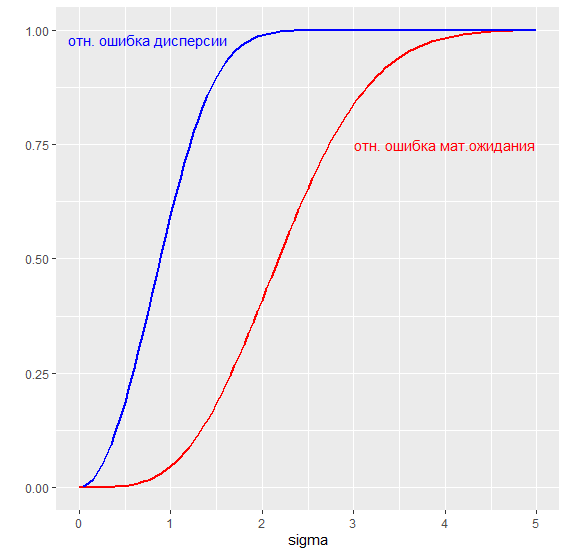
\includegraphics[width=1\linewidth]{img/par_new2.jpg}
				\caption{Ошибка аппроксимации мат. ожидания и дисперсии} %% подпись к рисунку
				\label{ris:image1} %% метка рисунка для ссылки на него
			\end{minipage}
			
		\end{center}
	\end{figure}
	
	\section{Произведение двух логнормальных распределений}
	Рассмотрим произведение логнормально распределенных случайных величин. Эта процедура применяется в нефтяной промышленности, например, используем площадь дренирования пласта, среднюю чистую толщину и коэффициент извлечения углеводородов. При перемножении этих параметров получаем количество резервов нефти. Идеи доказательств Предложений этого раздела взяты из статьи «Uncertainties impacting reserves, revenue, and costs» \cite{Uncertainties}.
	
	Мы рассмотрим произведение двух логнормально распределенных случайных величин 
	\begin{equation*}
		\ln(\xi_{1}) \sim N(\mu_{1}, \sigma _{1}^{2}),
	\end{equation*}
	\begin{equation*}
		\ln(\xi_{2}) \sim N(\mu_{2}, \sigma _{2}^{2}).
	\end{equation*}
	
	Введем следующие обозначения:\\
	$x_{\pi}$, $x_{0.5}$, $x_{1-\pi}$ "--- квантили случайной величины $\xi_{1}$,\\
	$y_{\pi}$, $y_{0.5}$, $y_{1-\pi}$ "--- квантили случайной величины $\xi_{2}$.
	
	\subsection{Произведение квантилей}
	\begin{proposition}
		Величина $x_{\pi}y_{\pi}$ является q-квантилью случайной величины $\xi_{1}\xi_{2}$, где
		
		\begin{equation}
			q = \mathsf{P}(\xi_{1}\xi_{2}< x_{\pi}y_{\pi}) =\Phi\left(\frac{\Phi^{-1}(\pi)(\ln(x_{0.5})+\ln(y_{0.5})-\ln(x_{\pi})-\ln(y_{\pi}))}{\sqrt{(\ln(x_{0.5})-\ln(x_{\pi}))^{2}+(\ln(y_{0.5})-\ln(y_{\pi}))^{2}}}\right). \label{20}
		\end{equation} 
	\end{proposition}
	\begin{Proof}
		Выразим параметры распределений $\mu_{1}$, $\mu_{2}$, $\sigma_{1}$, $\sigma_{2}$ через квантили, используя формулу \eqref{14}. Теперь рассмотрим случайную величину $\eta = \xi_{1}\xi_{2}$. Мы хотим вычислить, каким квантилем для $\eta$ является произведение квантилей $x_{\pi}$ и $y_{\pi}$. Для этого надо найти, чему равна вероятность $\mathsf{P}(\xi_{1}\xi_{2}< x_{\pi}y_{\pi})$. Получаем
		\begin{equation*}
			\mathsf{P}(\xi_{1}\xi_{2}< x_{\pi}y_{\pi}) = \mathsf{P}(\ln(\xi_{1})+\ln(\xi_{2})<\ln(x_{\pi})+\ln(y_{\pi}))=
		\end{equation*}
		\begin{equation*}
			=\mathsf{P}\left(\displaystyle{\frac{\ln(\xi_{1})+\ln(\xi_{2})-(\mu_{1}+\mu_{2})}{\sqrt{\sigma_{1}^{2}+\sigma_{2}^{2}}}}<\displaystyle{\frac{\ln(x_{\pi})+\ln(y_{\pi})-(\mu_{1}+\mu_{2})}{\sqrt{\sigma_{1}^{2}+\sigma_{2}^{2}}}}\right).
		\end{equation*}
		Так как $\xi_{1}$ распределена логнормально с параметрами $\mu_{1}$ и $\sigma_{1}^{2}$, а $\xi_{2}$ распределена логнормально с параметрами $\mu_{2}$ и $\sigma_{2}^{2}$, то
		\begin{equation*} 
			\ln(\xi_{1})+\ln(\xi_{2})\sim N(\mu_{1}+\mu_{2}, \sigma_{1}^{2}+\sigma_{2}^{2}),
		\end{equation*}
		\begin{equation*}
			\frac{\ln(\xi_{1})+\ln(\xi_{2})-(\mu_{1}+\mu_{2})}{\sqrt{\sigma_{1}^{2}+\sigma_{2}^{2}}} \sim N(0,1).
		\end{equation*}
		Тогда можно записать
		\begin{equation*}
			\mathsf{P}(\xi_{1}\xi_{2}< x_{\pi}y_{\pi}) =
		\end{equation*}
		\begin{equation*}
			=\mathsf{P}\left(\displaystyle{\frac{\ln(\xi_{1})+\ln(\xi_{2})-(\mu_{1}+\mu_{2})}{\sqrt{\sigma_{1}^{2}+\sigma_{2}^{2}}}}<\displaystyle{\frac{(\mu_{1}+\Phi^{-1}(\pi)\sigma_{1})+(\mu_{2}+\Phi^{-1}(\pi)\sigma_{2})-(\mu_{1}+\mu_{2})}{\sqrt{\sigma_{1}^{2}+\sigma_{2}^{2}}}}\right)=
		\end{equation*}
		
		\begin{equation*}
			=\mathsf{P}\left(\displaystyle{\frac{\ln(\xi_{1})+\ln(\xi_{2})-(\mu_{1}+\mu_{2})}{\sqrt{\sigma_{1}^{2}+\sigma_{2}^{2}}}}<\displaystyle{\frac{\Phi^{-1}(\pi)(\sigma_{1}+\sigma_{2})}{\sqrt{\sigma_{1}^{2}+\sigma_{2}^{2}}}}\right)=
		\end{equation*}
		\begin{equation*}
			=\Phi\left(\frac{\Phi^{-1}(\pi)(\sigma_{1}+\sigma_{2})}{\sqrt{\sigma_{1}^{2}+\sigma_{2}^{2}}}\right).
		\end{equation*}
		Перепишем эту дробь через значения квантилей, получаем
		\begin{align*}
			\frac{\Phi^{-1}(\pi)(\sigma_{1}+\sigma_{2})}{\sqrt{\sigma_{1}^{2}+\sigma_{2}^{2}}} &= \frac{\Phi^{-1}(\pi)\left(\displaystyle{\frac{(\ln(x_{0.5})-\ln(x_{\pi}))+(\ln(y_{0.5})-\ln(y_{\pi}))}{-\Phi^{-1}(\pi)}}\right)}{\sqrt{\dfrac{(\ln(x_{0.5})-\ln(x_{\pi}))^{2}+(\ln(y_{0.5})-\ln(y_{\pi}))^{2}}{(\Phi^{-1}(\pi))^{2}}}}=\\\\
			&=\dfrac{(\ln(x_{0.5})-\ln(x_{\pi}))+(\ln(y_{0.5})-\ln(y_{\pi}))}{\dfrac{\sqrt{(\ln(x_{0.5})-\ln(x_{\pi}))^{2}+(\ln(y_{0.5})-\ln(y_{\pi}))^{2}}}{\Phi^{-1}(\pi)}}.
		\end{align*}
		Тогда получаем следующую формулу
		\begin{equation*}
			\mathsf{P}(\xi_{1}\xi_{2}< x_{\pi}y_{\pi}) =\Phi\left(\frac{\Phi^{-1}(\pi)(\ln(x_{0.5})+\ln(y_{0.5})-\ln(x_{\pi})-\ln(y_{\pi}))}{\sqrt{(\ln(x_{0.5})-\ln(x_{\pi}))^{2}+(\ln(y_{0.5})-\ln(y_{\pi}))^{2}}}\right).
		\end{equation*}
		
	\end{Proof}
	
	\begin{corollary}
		При перемножение квантилей $x_{0.5}$ и $y_{0.5}$ получается снова 0.5-ый квантиль.   
	\end{corollary}
	\begin{Proof}
		Запишем вероятность $\mathsf{P}(\xi_{1} \xi_{2} < x_{0.5}y_{0.5})$ следующим образом:
		\begin{equation*}
			\mathsf{P}(\xi_{1} \xi_{2} < x_{0.5}y_{0.5}) =\Phi\left( \dfrac{\ln(x_{0.5})+\ln(y_{0.5}) - (\mu_{1}+\mu_{2})}{\sqrt{\sigma_{1}^{2}+\sigma_{2}^{2}}}\right).
		\end{equation*}
		Но в числителе получается 0, значит,
		\begin{equation*}
			\mathsf{P}(\xi_{1} \xi_{2} < x_{0.5}y_{0.5}) = \Phi(0) = 0.5.
		\end{equation*} 
	\end{Proof}
	
	\subsection{q-Квантили произведения логнормальных случайных величин для $q=\pi$, $q=0.5$, $q=1-\pi$}	
	Как по каким-то произвольным получившимся квантилям, полученным при перемножении данных квантилей для двух логнормальных случайных величин, найти нужные нам, такие же, как исходные $\pi$, $0.5$, $1-\pi$ квантили произведения этих двух случайных величин? Cначала нужно понять, на какой прямой лежат точки вида ($x_{\pi}$; $\Phi^{-1}(\pi)$).
	
	Нужно выяснить, как связаны параметры нормального распределения, квантили которого откладываются по оси $X$, и параметры прямой, на которой лежат точки QQ плота.
	
	\begin{proposition}
	Точки QQ-плота: $\left\{x_{i},\mathsf{F}_{\eta}^{-1}(\mathsf{F}_{\xi}(x_{i}))\right\}_{i=1}^{n}$, где
	ось $X$: $\xi \sim N(a, b^{2})$, ось $Y$: $\eta \sim N(0, 1)$
	лежат на прямой $y = \dfrac{x-a}{b}$.
	\end{proposition}
	\begin{Proof}
	Возьмем две точки и построим по ним уравнение прямой. Например, точки
	\[(\mathsf{F}_{\xi}^{-1}(0.1), \mathsf{F}_{\eta}^{-1}(0.1)),\]
	\[(\mathsf{F}_{\xi}^{-1}(0.5), \mathsf{F}_{\eta}^{-1}(0.5)).\]
	Имеем
	\begin{equation*}
		\Phi\left(\dfrac{x_{p}-a}{b}\right)=p\quad\quad \Rightarrow \quad\quad \dfrac{x_{p}-a}{b}=\Phi^{-1}(p).
	\end{equation*}
	Получаем, что
	\begin{equation*}
		x_{p}=a+b\Phi^{-1}(p).
	\end{equation*}
	Для первой точки возьмем $p = 0.1$, тогда
	\[(a+b\Phi^{-1}(0.1); \Phi^{-1}(0.1)).\]
	Для второй точки возьмем $p = 0.5$, тогда
	\[(a+b\Phi^{-1}(0.5); \Phi^{-1}(0.5)) \quad\quad \Rightarrow \quad\quad (a;0). \]
	Составим уравнение прямой:
	\[\dfrac{x-a}{(a+\Phi^{-1}(0.1)b)-a} = \dfrac{y}{\Phi^{-1}(0.1)}, \quad\quad\quad\quad \dfrac{x-a}{\Phi^{-1}(0.1)b} = \dfrac{y}{\Phi^{-1}(0.1)}.\]
	Следовательно,
	\begin{equation*} 
		by = x-a,
	\end{equation*}
	Получили уравнение прямой на которой лежат точки данного QQ-плота:
	\begin{equation*}
		y = \dfrac{x-a}{b}.
	\end{equation*}
\end{Proof}
	
	\begin{proposition}[\textbf{Swanson, 2000 год}]
		Зная квантили $x_{\pi}$, $x_{0.5}$, $x_{1-\pi}$ случайной величины $\xi_{1}$ и квантили $y_{\pi}$, $y_{0.5}$, $y_{1-\pi}$ случайной величины $\xi_{2}$, можно найти квантили $z_{\pi}$, $z_{0.5}$, $z_{1-\pi}$ случайной величины $\xi_{1}\xi_{2}$ как
		\begin{equation*}
			z_{\pi}=\exp(b\Phi^{-1}(\pi)+a),
		\end{equation*}
		\begin{equation*}
			z_{0.5}=x_{0.5}y_{0.5},
		\end{equation*}
		\begin{equation*}
			z_{1-\pi}=\exp(b\Phi^{-1}(1-\pi)+a),
		\end{equation*}
		где $a$ и $b$ такие, что прямая $y=\dfrac{x-a}{b}$ проходит через точки $(\ln(x_{\pi}y_{\pi}), t)$ и $(\ln(x_{0.5}y_{0.5}),0)$ при
		\begin{equation*}
			t = \frac{\Phi^{-1}(\pi)((\ln(x_{0.5})+\ln(y_{0.5}))-(\ln(x_{\pi})+\ln(y_{\pi})))}{\sqrt{(\ln(x_{0.5})-\ln(x_{\pi}))^{2}+(\ln(y_{0.5})-\ln(y_{\pi}))^{2}}}. 
		\end{equation*}
	\end{proposition}
	\begin{Proof}
		С помощью формулы \eqref{19} можно посчитать, какой получается квантиль для случайной величины $\xi_{1}\xi_{2}$, если перемножить квантили $x_{\pi}$ и $y_{\pi}$ исходных случайных величин. Обозначим $z_{\pi}$, $z_{0.5}$, $z_{1-\pi}$ "--- квантили случайной величины $\eta$. Тогда по Следствию 1 имеем $x_{0.5}y_{0.5} = z_{0.5}$.
		
		Нужно вычислить значения $z_{\pi}$ и $z_{1-\pi}$. Введем обозначение:
		\begin{equation*}
			t = \frac{\Phi^{-1}(\pi)((\ln(x_{0.5})+\ln(y_{0.5}))-(\ln(x_{\pi})+\ln(y_{\pi})))}{\sqrt{(\ln(x_{0.5})-\ln(x_{\pi}))^{2}+(\ln(y_{0.5})-\ln(y_{\pi}))^{2}}}. 
		\end{equation*}
		Тогда по Предложению 9 с помощью точек $(\ln(x_{\pi}y_{\pi}), t)$ и $(\ln(x_{0.5}y_{0.5}),0)$  можно найти параметры $a$ и $b$ прямой, на которой они лежат.
		
		\begin{equation*}
			\dfrac{\ln(x_{0.5}y_{0.5})-a}{b}=0 \quad\quad \Rightarrow \quad\quad a=\ln(x_{0.5}y_{0.5}),
		\end{equation*}
		
		\begin{equation*}
			\dfrac{\ln(x_{\pi}y_{\pi})-a}{b}=t,
		\end{equation*}
		
		\begin{equation*}
			b=\dfrac{\ln(x_{\pi}y_{\pi})-a}{t}=\dfrac{\ln(x_{\pi}y_{\pi})-\ln(x_{0.5}y_{0.5})}{t}.
		\end{equation*}
		Так как точки $(\ln(z_{\pi}), \Phi^{-1}(\pi))$ и $(\ln(z_{1-\pi}), \Phi^{-1}(1-\pi))$ тоже лежат на этой прямой, то мы можем вычислить значения $\ln(z_{\pi})$ и $\ln(z_{0.5})$, зная уравнение прямой, следующим образом:
		\begin{equation*}
			\dfrac{\ln(z_{\pi})-a}{b}=\Phi^{-1}(\pi),
		\end{equation*}
		\begin{equation*}
			\ln(z_{\pi})=b\Phi^{-1}(\pi)+a,
		\end{equation*}
		
		\begin{equation*}
			\dfrac{\ln(z_{1-\pi})-a}{b}=\Phi^{-1}(1-\pi),
		\end{equation*}
		\begin{equation*}
			\ln(z_{1-\pi})=b\Phi^{-1}(1-\pi)+a.
		\end{equation*}
		И, наконец, находим $z_{\pi}$ и $z_{1-\pi}$.
		\begin{equation*}
			z_{\pi}=\exp(b\Phi^{-1}(\pi)+a),
		\end{equation*}
		\begin{equation*}
			z_{1-\pi}=\exp(b\Phi^{-1}(1-\pi)+a).
		\end{equation*}
	\end{Proof}
	
	По Алгоритму 1, используя найденные $z_{\pi}$, $z_{0.5}$, $z_{1-\pi}$ , можно вычислить значения весов $p_{1}$, $p_{2}$, $p_{3}$ дискретной аппроксимации.
	
	\section{Сумма двух логнормальных распределений}
	
	Рассмотрим сумму двух логнормальных случайных величин.
	\begin{equation*}
		\ln(\xi_{1}) \sim N(\mu_{1}, \sigma _{1}^{2}),
	\end{equation*}
	\begin{equation*}
		\ln(\xi_{2}) \sim N(\mu_{2}, \sigma _{2}^{2}),
	\end{equation*}
	\begin{equation*}
		\xi = \xi_{1}+\xi_{2}.
	\end{equation*}
	
	Дано: квантили $x_{\pi}$, $x_{0.5}$, $x_{1-\pi}$ случайной величины $\xi_1$ и  квантили $y_{\pi}$, $y_{0.5}$, $y_{1-\pi}$ случайной величины $\xi_2$.
	
	Поставим задачу аппроксимации суммы логнормальным распределением $\ln(\eta) \sim N(\mu, \sigma^{2})$, так как нужно рассматривать сумму не обязательно двух, а произвольного числа случайных величин.
	
	Нужно найти квантили $z_{\pi}$, $z_{0.5}$, $z_{1-\pi}$ случайной величины $\eta$. По известным квантилям уже знаем, как вычислять вероятности $p_{1}$, $p_{2}$, $p_{3}$ такие, что $m = \tilde{m}$  и $s^{2} = \tilde{s}^{2}$.
	
	У нас есть следующие ограничения на параметры: $\mu_{1}, \mu_{2} < 12$, $\sigma_{1}, \sigma_{2} < 1.5$. Пусть мы нашли аппроксимацию суммы двух логнормальных величин, тогда с учетом этих ограничений её значения $\mu$ и $\sigma$ тоже будут иметь свои ограничения. При этом, чтобы найти значения вероятностей $p_{1}$, $p_{2}$, $p_{3}$ нужно, чтобы выполнялось то же условие, что в разделе 4.3. А именно, $\sigma < 0.6913.$
	
	Имеем следующий алгоритм для решения задачи.
	
	\begin{alg}\label{al3}
		\begin{pr1}
			Квантили $x_{\pi}$, $x_{0.5}$, $x_{1-\pi}$ "--- квантили $\xi_{1}$, $y_{\pi}$, $y_{0.5}$, $y_{1-\pi}$ "--- квантили $\xi_{2}$.
		\end{pr1}
		\begin{enumerate}
			\item $x_{\pi}$, $x_{0.5}$, $x_{1-\pi}$ $\rightarrow$  $\mu_{1}$, $\sigma_{1}$
			
			По набору квантилей $\xi_{1}$ находим параметры $\mu_{1}$, $\sigma_{1}$ нормального распределения по формулам \eqref{13} и \eqref{14}.
			\item $y_{\pi}$, $y_{0.5}$, $y_{1-\pi}$ $\rightarrow$ $\mu_{2}$, $\sigma_{2}$
			
			По набору квантилей $\xi_{2}$ находим параметры $\mu_{2}$, $\sigma_{2}$ нормального распределения по формулам \eqref{13} и \eqref{14}.
			\item $\mu_{i}$, $\sigma_{i}$ $\rightarrow$ $m_{i}$, $s_{i}^{2}$
			
			С помощью формул \eqref{8} и \eqref{9} находим мат. ожидания и дисперсии $\xi_{1}$ и $\xi_{2}.$
			\item $m = m_{1}+m_{2}$
			
			Вычисляем мат.ожидание $\xi_{1}+\xi_{2}.$
			\item $s^{2}=s_{1}^{2} + s_{2}^{2}$
			
			Вычисляем дисперсию $\xi_{1}+\xi_{2}.$
			\item $m$, $s^{2}$ $\rightarrow$ $\mu$, $\sigma$
			
			С помощью формул \eqref{8} и \eqref{9} находим параметры нормального распределения.
			\item $\mu$, $\sigma$ $\rightarrow$ $z_{\pi}$, $z_{0.5}$, $z_{1-\pi}$
			
			С помощью формулы \eqref{14} находим значения квантилей через $\mu$ и $\sigma$.
			\item $z_{\pi}$, $z_{0.5}$, $z_{1-\pi}$ $\rightarrow$ $p_{1}$, $p_{2}$, $p_{3}$
			
			По Алгоритму 1 находим значения вероятностей $p_{1}$, $p_{2}$, $p_{3}$.
		\end{enumerate}
		
		\begin{pr3}\end{pr3} вероятности $p_{1}$, $p_{2}$, $p_{3}$ для квантилей $z_{\pi_{1}}, z_{\pi_{2}}, z_{\pi_{3}}$ случайной величины $\eta$, которая является дискретной аппроксимацией аппроксимации суммы логнормальным распределением.
		
	\end{alg}
	
	\paragraph{Точность аппроксимации.}
	
	Выразим ошибки аппроксимации квантилей $q_{\pi}$, $q_{0.5}$, $q_{1-\pi}$ случайной величины $\xi$ через параметры $\mu_{1}$, $\mu_{2}$, $\sigma_{1}^{2}$, $\sigma_{2}^{2}$.
	
	\[\dfrac{\left| q_{\pi} - z_{\pi}\right|}{q_{\pi}}, \quad\quad \dfrac{\left| q_{0.5} - z_{0.5}\right|}{q_{0.5}}, \quad\quad \dfrac{\left| q_{1-\pi} - z_{1-\pi}\right|}{q_{1-\pi}}.\]
	
	\[z_{\pi} = F_{\eta}^{-1}(\pi), \quad\quad z_{0.5} = \exp(\mu), \quad\quad z_{1-\pi} = F_{\eta}^{-1}(1-\pi), \quad где\]
	\[F_{\eta}^{-1}(p) = \exp(\mu+\sigma\sqrt{2}\mathrm{erf}^{-1}(2p-1)).\]
	Параметры $\mu$, $\sigma$ можно найти через параметры случайных величин $\xi_{1}$, $\xi_{2}$, используя формулы \eqref{8}, \eqref{9} и вычисленные значения
	\[m = \exp\left( \mu_{1}+\frac{\sigma_{1}^{2}}{2}\right) + \exp\left( \mu_{2}+\frac{\sigma_{2} ^{2}}{2}\right),\]
	\[s^{2} = m_{1}^{2}(\exp(\sigma_{1}^{2})-1)+m_{2}^{2}(\exp(\sigma_{2}^{2})-1).\]
	Квантили $\eta$ выражаются как
	\[q_{\pi} = F_{\xi}^{-1}(\pi), \quad\quad q_{0.5} = F_{\xi}^{-1}(0.5), \quad\quad q_{1-\pi} = F_{\xi}^{-1}(1-\pi), \quad где\]
	\[F_{\xi}(x) = \int_{0}^{x}\left( \dfrac{1}{2}+\dfrac{1}{2} \mathrm{erf}\left( \dfrac{\ln(x-y)-\mu_{1}}{\sigma_{1}\sqrt{2}}\right) \right) \left( \dfrac{1}{\sqrt{2\pi}y\sigma_{2}}\exp\left( -\left( \dfrac{\ln(y)-\mu_{2}}{\sqrt{2}\sigma_{2}}\right) ^{2}\right) \right) dy. \]
	Здесь $F_{\xi}(x)$ "--- функция распределения $\xi = \xi_{1}+\xi_{2}$, найденная с помощью формулы свертки.
	
	В таблицах \ref{tab1}, \ref{tab2} и \ref{tab3} представлены ошибки для $\ln(\xi_{1}) \sim N(4, \sigma _{1}^{2})$, $\ln(\xi_{2}) \sim N(4, \sigma_{2}^{2})$ при $\pi=0.1$, полученные с помощью моделирования, объемы выборок равны $10^{6}$. По построению аппроксимации суммы двух логнормальных распределений логнормальным распределением ошибки мат. ожидания и дисперсии равны 0, то есть $m=\tilde{m}$ и $s^{2} = \tilde{s}^{2}$. Но если для каких-либо расчетов понадобятся квантили $\eta$, то ошибка медианы может достигать 21\%, ошибка  квантиля $q_{10}$ достигает 67\%, ошибка квантиля $q_{90}$ достигает 20\%.
	
	%\centering
	%\textbf{$\sigma_{1}^{2}$, $\sigma_{2}^{2}$}
	%\backslashbox{два}{один} 
	
	\begin{table}[!hhh]
		\centering
		\caption{Ошибка аппроксимации медианы ($\%$) в зависимости от $\sigma_{1}^{2}$ (строка) и $\sigma_{2}^{2}$ (столбец) при $\mu_{1} = \mu_{2} = 4$.}
		\label{tab1}
		\begin{tabular}{rrrrrr}
			\hline
			& \textbf{0.25} & \textbf{0.75} & \textbf{1.25} & \textbf{1.75} & \textbf{2.25} \\ 
			\hline
			\textbf{0.25} & 0.24 & 0.46 & 4.19 & 11.67 & 21.10 \\ 
			\textbf{0.75} & 0.74 & 0.40 & 3.06 & 11.46 & 20.99 \\ 
			\textbf{1.25} & 4.25 & 3.27 & 2.48 & 6.18 & 16.15 \\ 
			\textbf{1.75} & 12.18 & 10.12 & 5.57 & 5.24 & 9.92 \\ 
			\textbf{2.25} & 20.94 & 20.20 & 16.29 & 9.59 & 8.47 \\ 
			\hline
		\end{tabular}
	\end{table}

\begin{table}[!hhh]
	\centering
	\caption{Ошибка аппроксимации $q_{10}$ ($\%$) в зависимости от $\sigma_{1}^{2}$ (строка) и $\sigma_{2}^{2}$ (столбец) при $\mu_{1} = \mu_{2} = 4$.}
	\label{tab2}
	\begin{tabular}{rrrrrr}
		\hline
		& \textbf{0.25} & \textbf{0.75} & \textbf{1.25} & \textbf{1.75} & \textbf{2.25} \\ 
		\hline
		\textbf{0.25} & 0.72 & 12.75 & 33.79 & 52.58 & 66.98 \\ 
		\textbf{0.75} & 12.30 & 3.81 & 15.13 & 35.85 & 53.91 \\ 
		\textbf{1.25} & 33.42 & 14.81 & 10.81 & 22.58 & 40.49 \\ 
		\textbf{1.75} & 52.84 & 35.57 & 19.95 & 18.15 & 27.68 \\ 
		\textbf{2.25} & 66.40 & 53.63 & 41.42 & 26.75 & 24.57 \\ 
		\hline
	\end{tabular}
\end{table}

\begin{table}[!hhh]
	\centering
	\caption{Ошибка аппроксимации $q_{90}$ ($\%$) в зависимости от $\sigma_{1}^{2}$ (строка) и $\sigma_{2}^{2}$ (столбец) при $\mu_{1} = \mu_{2} = 4$.}
	\label{tab3}
	\begin{tabular}{rrrrrr}
		\hline
		& \textbf{0.25} & \textbf{0.75} & \textbf{1.25} & \textbf{1.75} & \textbf{2.25} \\ 
		\hline
		\textbf{0.25} & 0.16 & 5.03 & 13.69 & 17.74 & 19.37 \\ 
		\textbf{0.75} & 5.63 & 1.89 & 5.77 & 10.70 & 16.03 \\ 
		\textbf{1.25} & 13.55 & 5.75 & 2.52 & 6.00 & 9.79 \\ 
		\textbf{1.75} & 19.95 & 11.88 & 5.77 & 3.50 & 4.89 \\ 
		\textbf{2.25} & 18.47 & 15.44 & 9.42 & 5.50 & 5.27 \\ 
		\hline
	\end{tabular}
\end{table}
	
	
	
	Построим графики 2, 3 и 4 зависимости ошибки аппроксимации квантилей от $\sigma_{2}^{2}$ при фиксированной $\sigma_{1}^{2} = 0.45$. При моделировании объемы выборок равны $10^{6}$.
	
	\begin{figure}[!hhh]
		\begin{center}
			\begin{minipage}[h]{0.8\linewidth}
				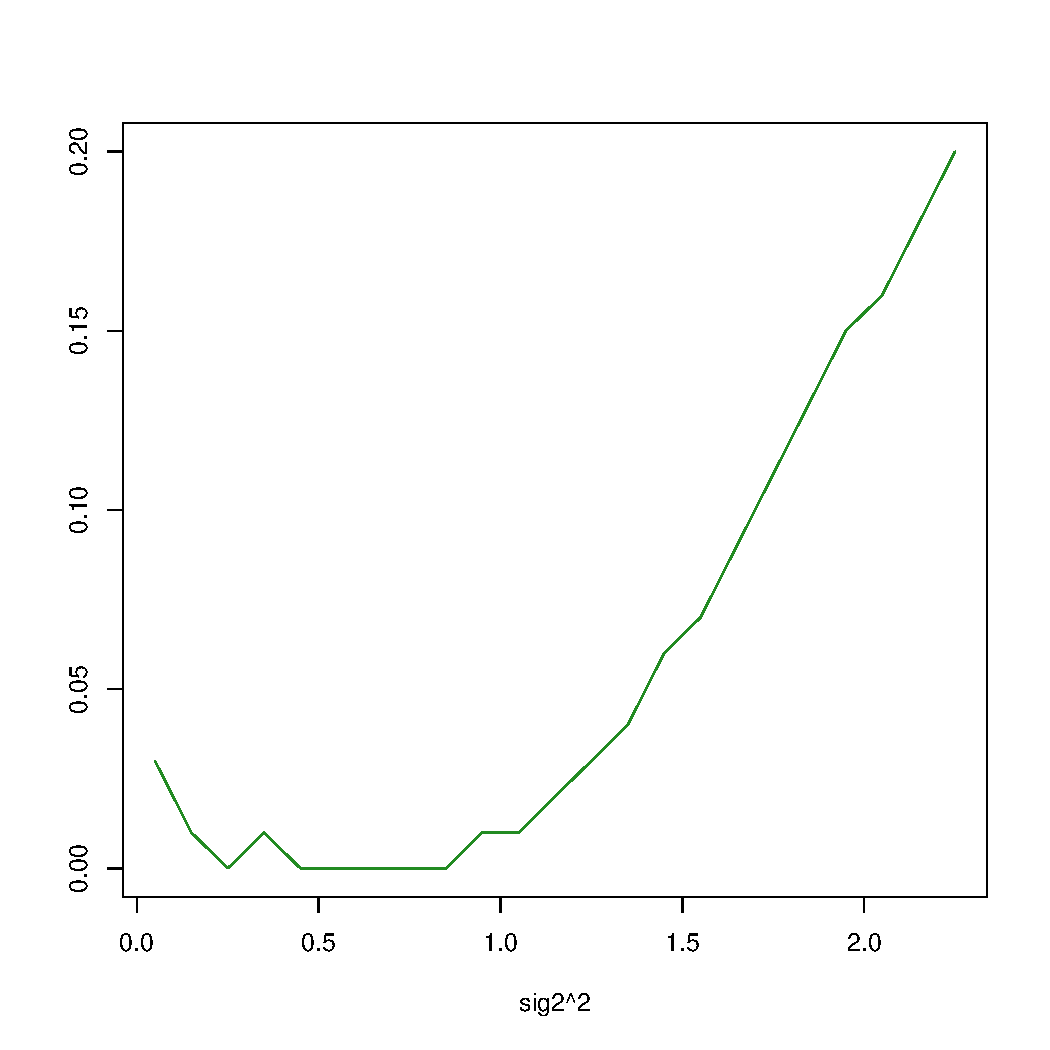
\includegraphics[width=1\linewidth]{img/gr_neww_1.pdf}
				\caption{Ошибка аппроксимации медианы при $\sigma_{1}^{2} = 0.75$.} %% подпись к рисунку
				\label{ris7} %% метка рисунка для ссылки на него
			\end{minipage}	
		\end{center}
	\end{figure}

\begin{figure}[!hhh]
	\begin{center}
		\begin{minipage}[h]{0.8\linewidth}
			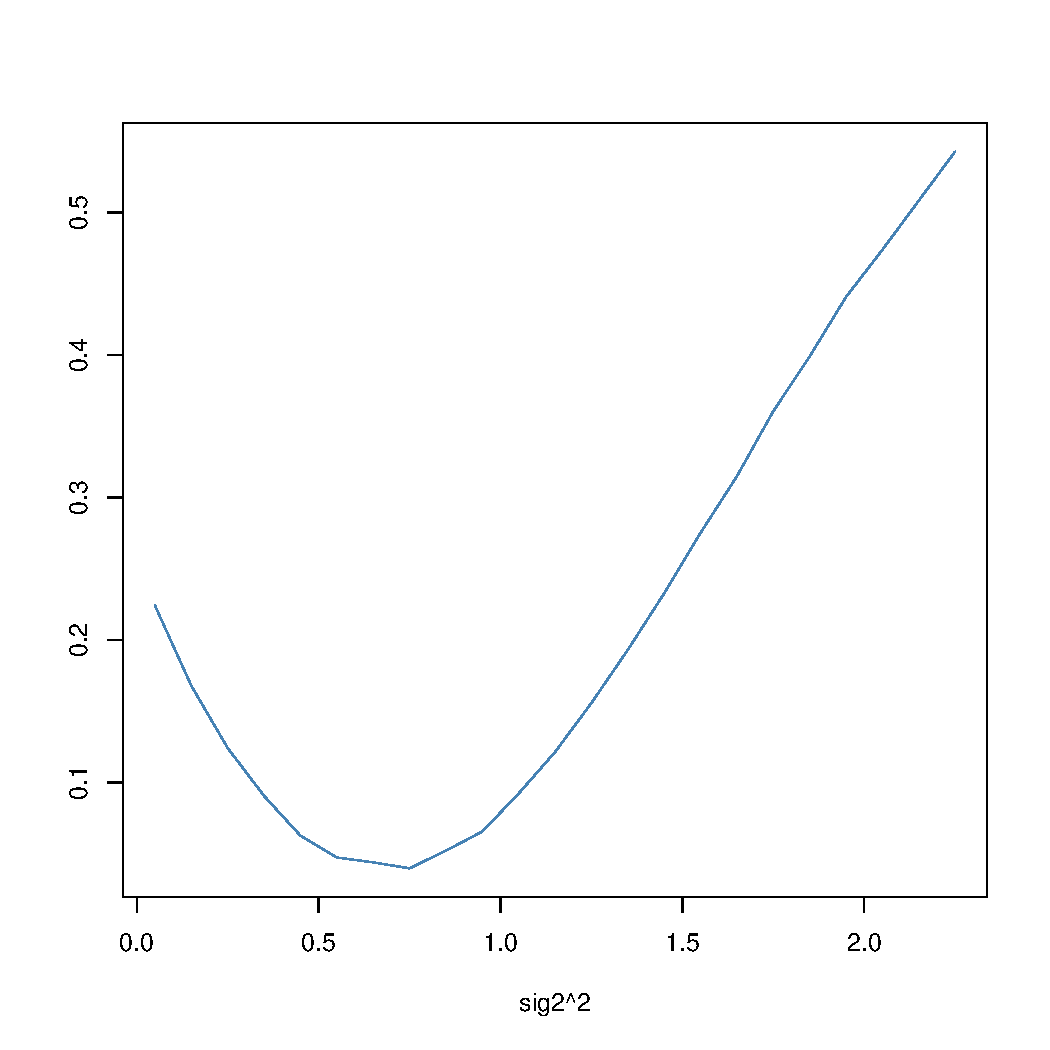
\includegraphics[width=1\linewidth]{img/gr_neww_2.pdf}
			\caption{Ошибка аппроксимации $q_{10}$ при $\sigma_{1}^{2} = 0.75$.} %% подпись к рисунку
			\label{ris8} %% метка рисунка для ссылки на него
		\end{minipage}	
	\end{center}
\end{figure}

\begin{figure}[!hhh]
	\begin{center}
		\begin{minipage}[h]{0.8\linewidth}
			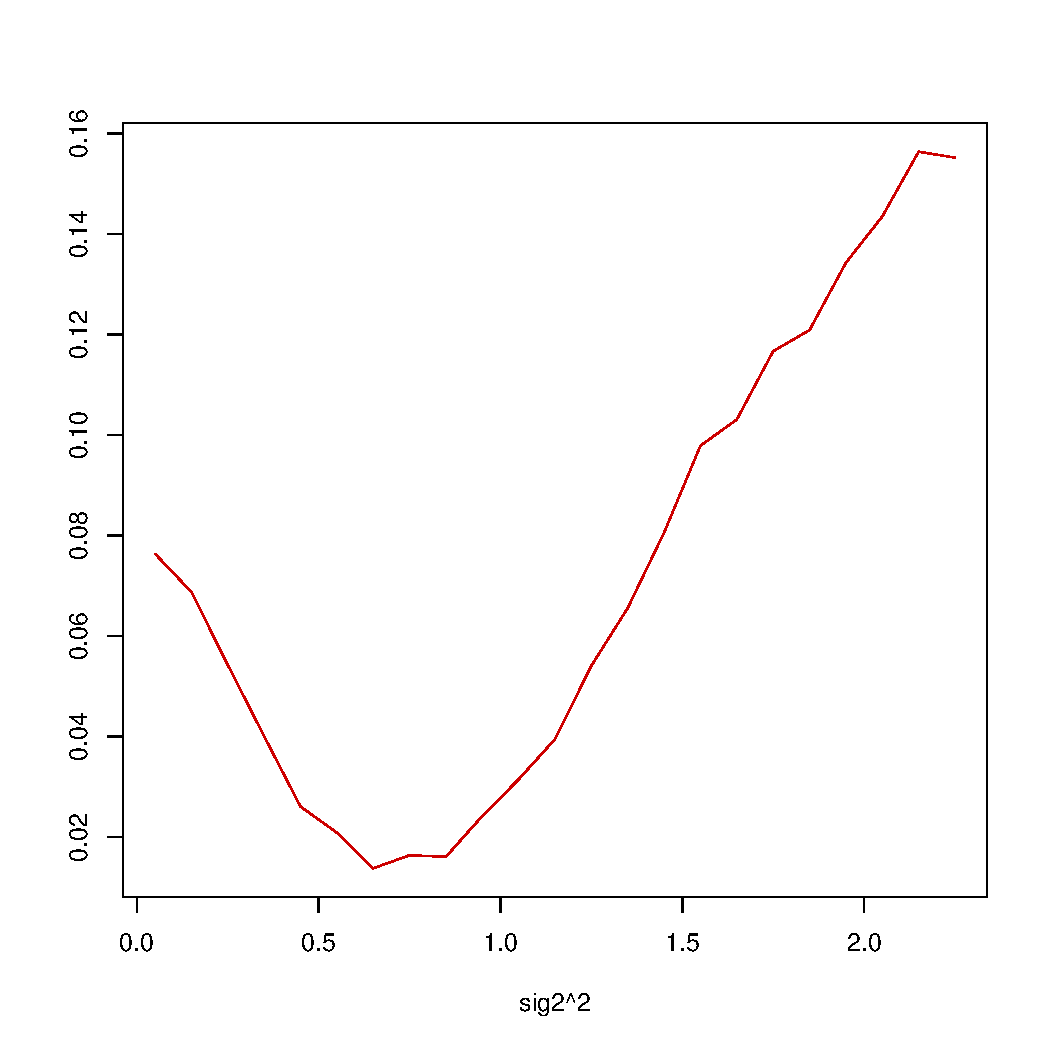
\includegraphics[width=1\linewidth]{img/gr_neww_3.pdf}
			\caption{Ошибка аппроксимации $q_{90}$ при $\sigma_{1}^{2} = 0.75$.} %% подпись к рисунку
			\label{ris9} %% метка рисунка для ссылки на него
		\end{minipage}	
	\end{center}
\end{figure}
	
	
	\begin{table}[!hhh]
		\centering
		\caption{$F_{\eta}(z_{50})$ ($\%$) в зависимости от $\sigma_{1}^{2}$ (строка) и $\sigma_{2}^{2}$ (столбец) при $\mu_{1} = \mu_{2} = 4$. }
		\label{tab4}
		\begin{tabular}{rrrrrr}
			\hline
			& \textbf{0.25} & \textbf{0.75} & \textbf{1.25} & \textbf{1.75} & \textbf{2.25} \\ 
			\hline
			\textbf{0.25} & 50.10 & 49.87 & 46.96 & 42.18 & 36.95 \\ 
			\textbf{0.75} & 49.87 & 49.82 & 48.30 & 44.55 & 39.74 \\ 
			\textbf{1.25} & 46.96 & 48.30 & 49.00 & 47.19 & 43.31 \\ 
			\textbf{1.75} & 42.18 & 44.55 & 47.19 & 47.91 & 46.03 \\ 
			\textbf{2.25} & 36.95 & 39.74 & 43.31 & 46.03 & 46.73 \\ 
			\hline
		\end{tabular}
	\end{table}

\begin{table}[!hhh]
	\centering
	\caption{$F_{\eta}(z_{10})$ ($\%$) в зависимости от $\sigma_{1}^{2}$ (строка) и $\sigma_{2}^{2}$ (столбец) при $\mu_{1} = \mu_{2} = 4$. }
	\label{tab5}
	\begin{tabular}{rrrrrr}
		\hline
		& \textbf{0.25} & \textbf{0.75} & \textbf{1.25} & \textbf{1.75} & \textbf{2.25} \\ 
		\hline
		\textbf{0.25} & 9.79 & 5.84 & 1.82 & 0.32 & 0.04 \\ 
		\textbf{0.75} & 5.84 & 8.89 & 6.45 & 3.14 & 1.19 \\ 
		\textbf{1.25} & 1.82 & 6.45 & 7.85 & 6.00 & 3.35 \\ 
		\textbf{1.75} & 0.32 & 3.14 & 6.00 & 6.89 & 5.43 \\ 
		\textbf{2.25} & 0.04 & 1.19 & 3.35 & 5.43 & 6.08 \\ 
		\hline
	\end{tabular}
\end{table}

\begin{table}[!hhh]
	\centering
	\caption{$F_{\eta}(z_{90})$ ($\%$) в зависимости от $\sigma_{1}^{2}$ (строка) и $\sigma_{2}^{2}$ (столбец) при $\mu_{1} = \mu_{2} = 4$.}
	\label{tab6}
	\begin{tabular}{rrrrrr}
		\hline
		& \textbf{0.25} & \textbf{0.75} & \textbf{1.25} & \textbf{1.75} & \textbf{2.25} \\
		\hline
		\textbf{0.25} & 90.08 & 91.47 & 92.31 & 92.42 & 92.19 \\ 
		\textbf{0.75} & 91.47 & 90.38 & 91.11 & 91.83 & 92.02 \\ 
		\textbf{1.25} & 92.31 & 91.11 & 90.57 & 90.93 & 91.31 \\ 
		\textbf{1.75} & 92.42 & 91.83 & 90.93 & 90.62 & 90.75 \\ 
		\textbf{2.25} & 92.19 & 92.02 & 91.31 & 90.75 & 90.56 \\ 
		\hline
	\end{tabular}
\end{table}	
	
	Теперь посчитаем значения функции $F_{\xi}(x)$ от квантилей $z_{10}$, $z_{50}$, $z_{90}$ случайной величины $\eta$. Они показывают, каким квантилем для $\xi$ являются квантили $z_{i}$. Результаты приведены в таблицаx \ref{tab4}, \ref{tab5} и \ref{tab6}.
	
	Построим оценки плотности для $\xi$ и $\eta$, когда ошибки имеют очень маленькие значения и когда достаточно большие. Они представлены на рисунках 5 и 6.
	
	\begin{figure}[!hhh]
		\begin{center}
			\begin{minipage}[h]{0.95\linewidth}
				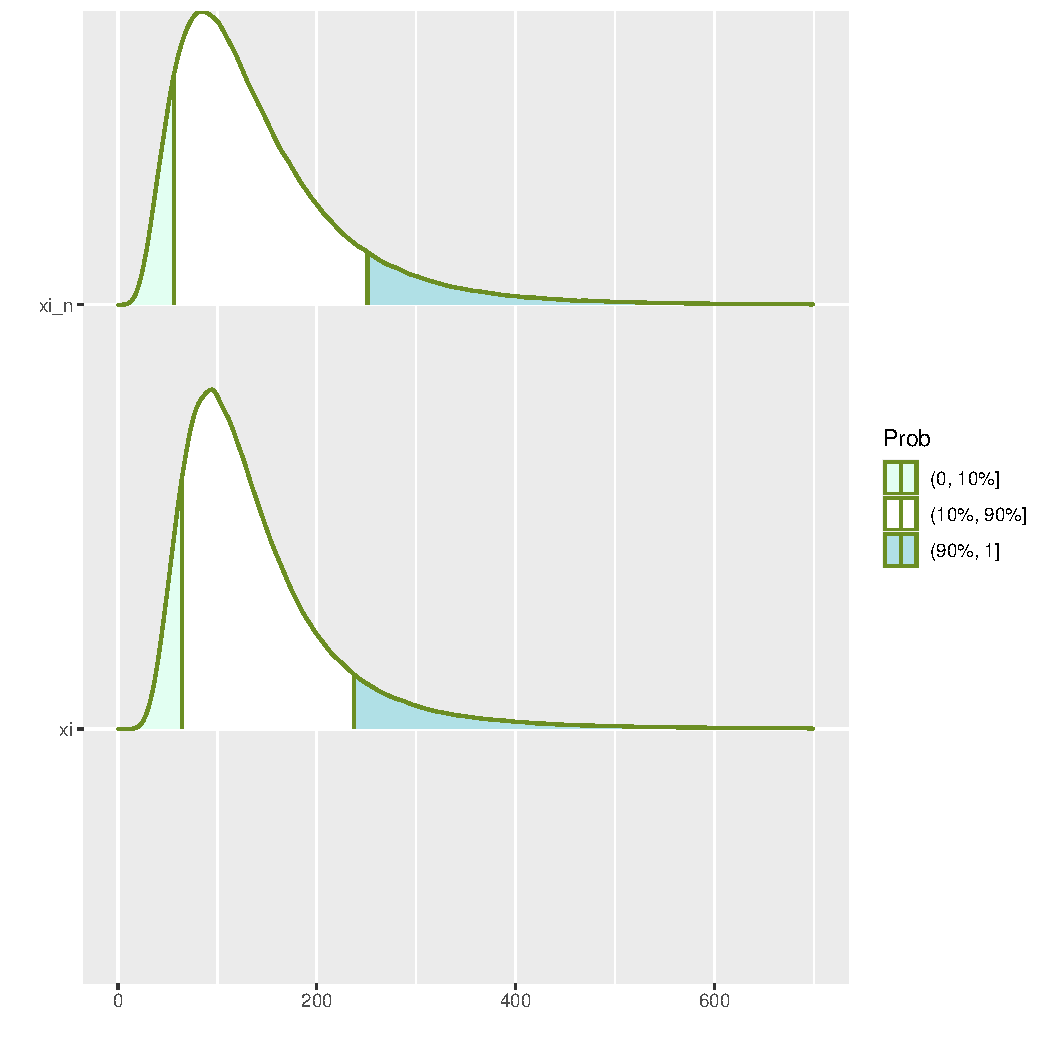
\includegraphics[width=1\linewidth]{img/sr1.pdf}
				\caption{$\sigma_{1}^{2} = 0.25$, $\sigma_{2}^{2} = 0.25$, $err_{med}$ = 0.17\%,  $err_{q_{10}} = 0.35\%$,  $err_{q_{90}} = 0.12\%$. } %% подпись к рисунку
				\label{ris5} %% метка рисунка для ссылки на него
			\end{minipage}
			
		\end{center}
	\end{figure}

\begin{figure}[!hhh]
	\begin{center}
		\begin{minipage}[h]{0.95\linewidth}
			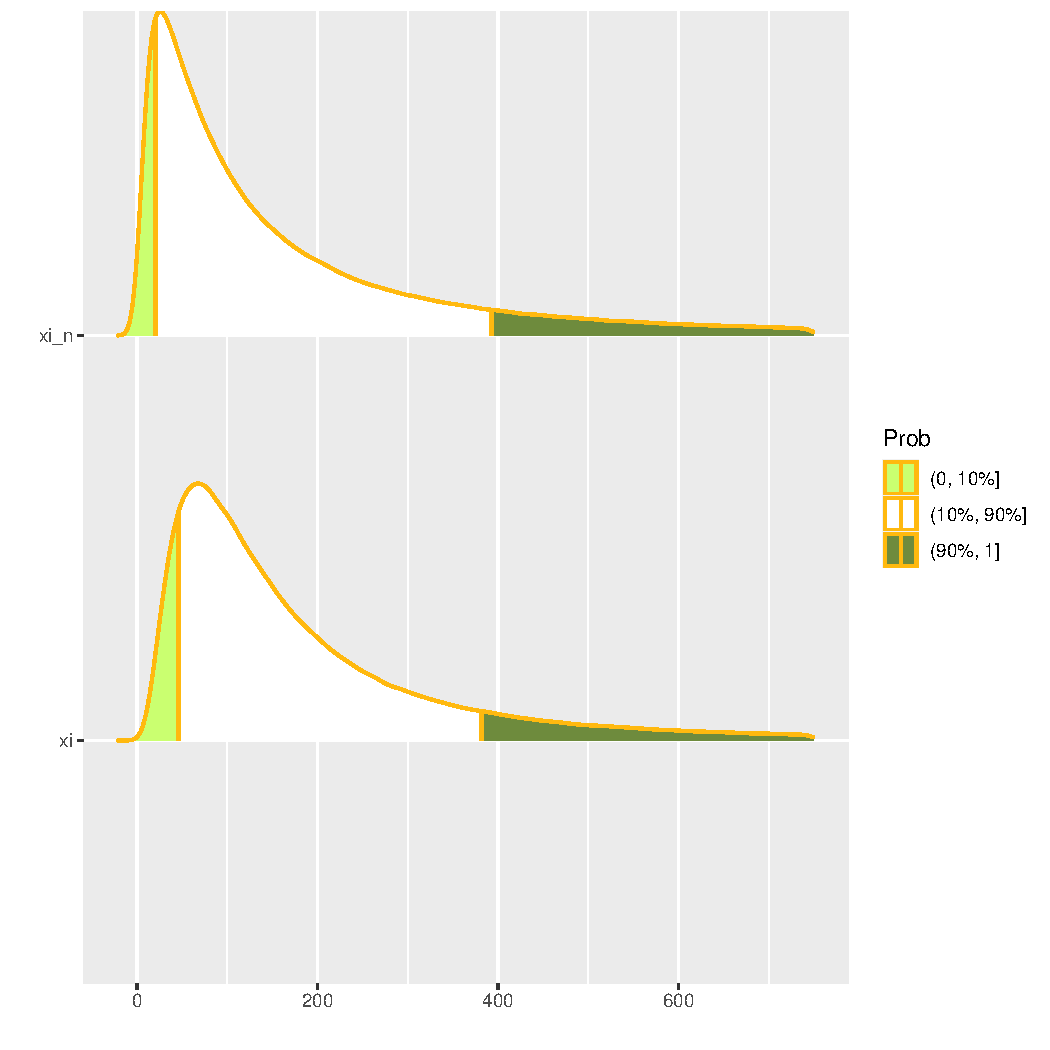
\includegraphics[width=1\linewidth]{img/sr2.pdf}
			\caption{$\sigma_{1}^{2} = 2.25$, $\sigma_{2}^{2} = 0.75$, $err_{med}$ = 20.4\%,  $err_{q_{10}} = 54.13\%$,  $err_{q_{90}} = 15.54\%$. } %% подпись к рисунку
			\label{ris6} %% метка рисунка для ссылки на него
		\end{minipage}
		
	\end{center}
\end{figure}

Также посмотрим на таблицы с коэффициентами асимметрии и эксцесса.

\begin{table}[!hhh]
	\centering
	\caption{Коэффициент асимметрии суммы (голубой) и аппроксимации (розовый) в зависимости от $\sigma_{1}^{2}$ (строка) и $\sigma_{2}^{2}$ (столбец) при $\mu_{1} = \mu_{2} = 4$.}
	\begin{tabular}{|c|l|l|l|l|l|}
		\hline
		& \textbf{0.25} & \textbf{0.75} & \textbf{1.25} & \textbf{1.75} & \textbf{2.5} \\ \hline
		\multirow{2}{*}{\textbf{0.25}} & \textcolor{cyan}{1.77}          & \textcolor{cyan}{4.23}          & \textcolor{cyan}{6.71}          & \textcolor{cyan}{15.59}         & \textcolor{cyan}{16.68}        \\ \cline{2-6} 
		& \textcolor{magenta}{1.53}          & \textcolor{magenta}{3.75}          & \textcolor{magenta}{7.48}          & \textcolor{magenta}{14.76}         & \textcolor{magenta}{29.70}        \\ \hline
		\multirow{2}{*}{\textbf{0.75}} & \textcolor{cyan}{1.66}          & \textcolor{cyan}{3.86}          & \textcolor{cyan}{7.39}          & \textcolor{cyan}{11.43}         & \textcolor{cyan}{54.43}        \\ \cline{2-6} 
		& \textcolor{magenta}{1.55}          & \textcolor{magenta}{3.65}          & \textcolor{magenta}{7.22}          & \textcolor{magenta}{14.25}         & \textcolor{magenta}{28.77}        \\ \hline
		\multirow{2}{*}{\textbf{1.25}} & \textcolor{cyan}{2.13}          & \textcolor{cyan}{3.68}          & \textcolor{cyan}{8.73}          & \textcolor{cyan}{13.76}         & \textcolor{cyan}{29.28}        \\ \cline{2-6} 
		& \textcolor{magenta}{1.71}          & \textcolor{magenta}{3.60}          & \textcolor{magenta}{6.97}          & \textcolor{magenta}{13.68}         & \textcolor{magenta}{27.66}        \\ \hline
		\multirow{2}{*}{\textbf{1.75}} & \textcolor{cyan}{5.88}          & \textcolor{cyan}{4.06}          & \textcolor{cyan}{7.50}          & \textcolor{cyan}{31.50}         & \textcolor{cyan}{24.89}        \\ \cline{2-6} 
		& \textcolor{magenta}{2.17}          & \textcolor{magenta}{3.71}          & \textcolor{magenta}{6.79}          & \textcolor{magenta}{13.09}         & \textcolor{magenta}{26.41}        \\ \hline
		\multirow{2}{*}{\textbf{2.5}}  & \textcolor{cyan}{11.18}         & \textcolor{cyan}{8.85}          & \textcolor{cyan}{8.55}          & \textcolor{cyan}{10.34}         & \textcolor{cyan}{23.61}        \\ \cline{2-6} 
		& \textcolor{magenta}{3.30}          & \textcolor{magenta}{4.29}          & \textcolor{magenta}{6.90}          & \textcolor{magenta}{12.66}         & \textcolor{magenta}{25.13}        \\ \hline
	\end{tabular}
\end{table}

\begin{table}[!hhh]
	\centering
	\caption{Коэффициент эксцесса суммы (голубой) и аппроксимации (розовый) в зависимости от $\sigma_{1}^{2}$ (строка) и $\sigma_{2}^{2}$ (столбец) при $\mu_{1} = \mu_{2} = 4$. }
	\begin{tabular}{|c|l|l|l|l|l|}
		\hline
		& \textbf{0.25} & \textbf{0.75} & \textbf{1.25} & \textbf{1.75} & \textbf{2.5} \\ \hline
		\multirow{2}{*}{\textbf{0.25}} & \textcolor{cyan}{6.54}          & \textcolor{cyan}{51.70}         & \textcolor{cyan}{227.68}        & \textcolor{cyan}{408.58}        & \textcolor{cyan}{734.47}       \\ \cline{2-6} 
		& \textcolor{magenta}{4.42}          & \textcolor{magenta}{32.60}         & \textcolor{magenta}{180.39}        & \textcolor{magenta}{1088.57}       & \textcolor{magenta}{7274.56}      \\ \hline
		\multirow{2}{*}{\textbf{0.75}} & \textcolor{cyan}{6.21}          & \textcolor{cyan}{61.66}         & \textcolor{cyan}{144.59}        & \textcolor{cyan}{201.69}        & \textcolor{cyan}{1304.88}      \\ \cline{2-6} 
		& \textcolor{magenta}{4.56}          & \textcolor{magenta}{30.53}         & \textcolor{magenta}{164.86}        & \textcolor{magenta}{990.42}        & \textcolor{magenta}{6666.16}      \\ \hline
		\multirow{2}{*}{\textbf{1.25}} & \textcolor{cyan}{11.47}         & \textcolor{cyan}{27.75}         & \textcolor{cyan}{179.22}        & \textcolor{cyan}{193.95}        & \textcolor{cyan}{546.57}       \\ \cline{2-6} 
		& \textcolor{magenta}{5.61}          & \textcolor{magenta}{29.53}         & \textcolor{magenta}{150.21}        & \textcolor{magenta}{886.71}        & \textcolor{magenta}{5989.44}      \\ \hline
		\multirow{2}{*}{\textbf{1.75}} & \textcolor{cyan}{122.65}        & \textcolor{cyan}{46.01}         & \textcolor{cyan}{110.03}        & \textcolor{cyan}{276.24}        & \textcolor{cyan}{14081.05}     \\ \cline{2-6} 
		& \textcolor{magenta}{9.44}          & \textcolor{magenta}{31.88}         & \textcolor{magenta}{140.69}        & \textcolor{magenta}{788.78}        & \textcolor{magenta}{5280.07}      \\ \hline
		\multirow{2}{*}{\textbf{2.5}}  & \textcolor{cyan}{195.77}        & \textcolor{cyan}{283.81}        & \textcolor{cyan}{344.56}        & \textcolor{cyan}{4837.85}       & \textcolor{cyan}{1292.23}      \\ \cline{2-6} 
		& \textcolor{magenta}{24.08}         & \textcolor{magenta}{44.88}         & \textcolor{magenta}{146.68}        & \textcolor{magenta}{720.26}        & \textcolor{magenta}{4612.33}      \\ \hline
	\end{tabular}
\end{table}

\section{Трехточечная несимметричная аппроксимация логнормального распределения}

Рассмотрим трехточечную аппроксимацию логнормального распределения с несимметричными квантилями. Пусть $\pi_{1} = 0.1$, $\pi_{2} = 0.5$. Посмотрим, как меняются вероятности $p_{1}$, $p_{2}$, $p_{3}$ в зависимости от $\pi_{3} = \pi$. 
\begin{figure}[!hhh]
	\begin{center}
		\begin{minipage}[h]{0.95\linewidth}
			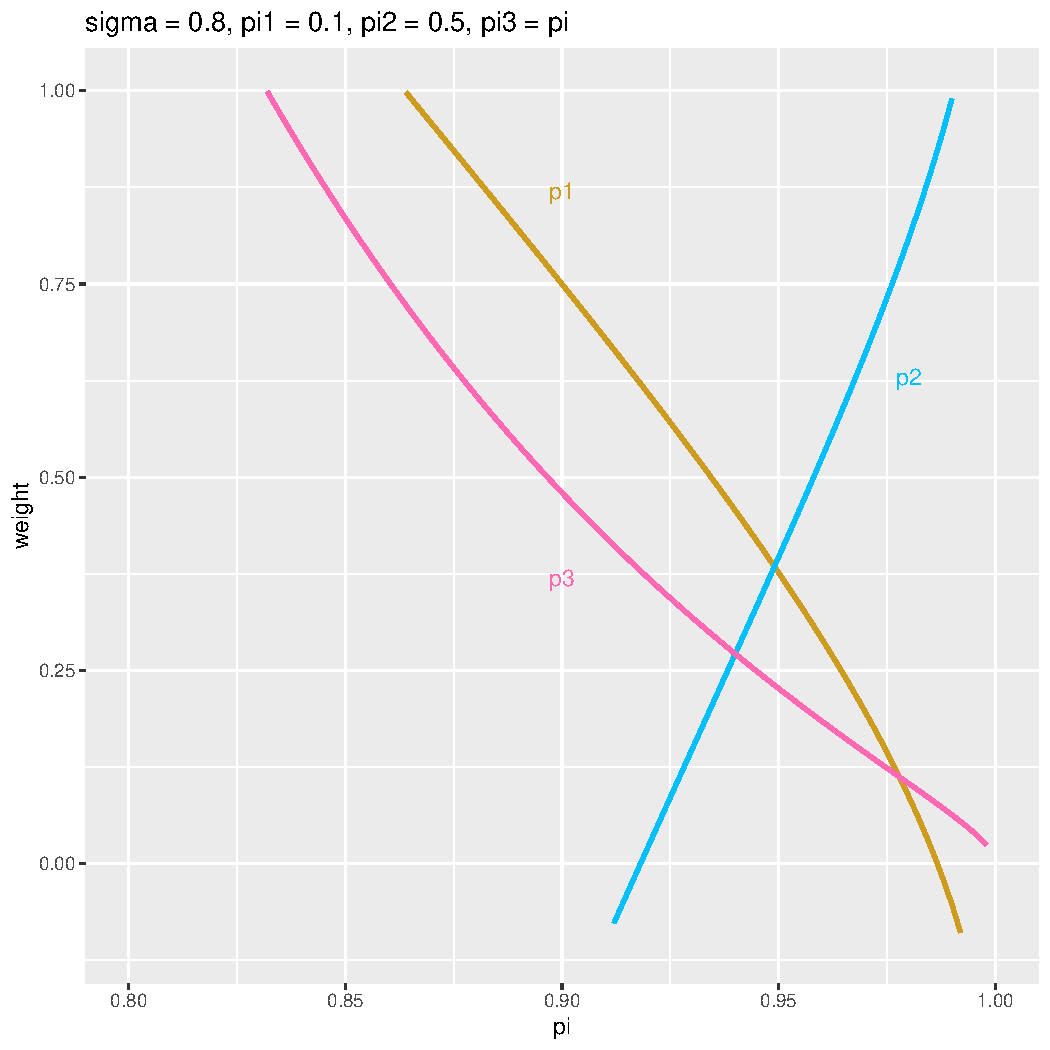
\includegraphics[width=1\linewidth]{img/p123_1.pdf}
			\caption{Веса $p_{1}$, $p_{2}$, $p_{3}$ в зависимости от $\pi$. } %% подпись к рисунку
			\label{ris10} %% метка рисунка для ссылки на него
		\end{minipage}
	\end{center}
\end{figure}
На графике 7 веса, найденные при $\sigma = 0.8$. Видим, что веса являются вероятностями при  $0.92 \leq \pi \leq 0.98$.

Теперь пусть $\pi_{1} = 0.1$, $\pi_{2} = \pi$, $\pi_{3} = 0.9$. На рисунке 8 видим, что при любом $\pi$ значение $p_{2}$ будет отрицательным.

\begin{figure}[!hhh]
	\begin{center}
		\begin{minipage}[h]{0.95\linewidth}
			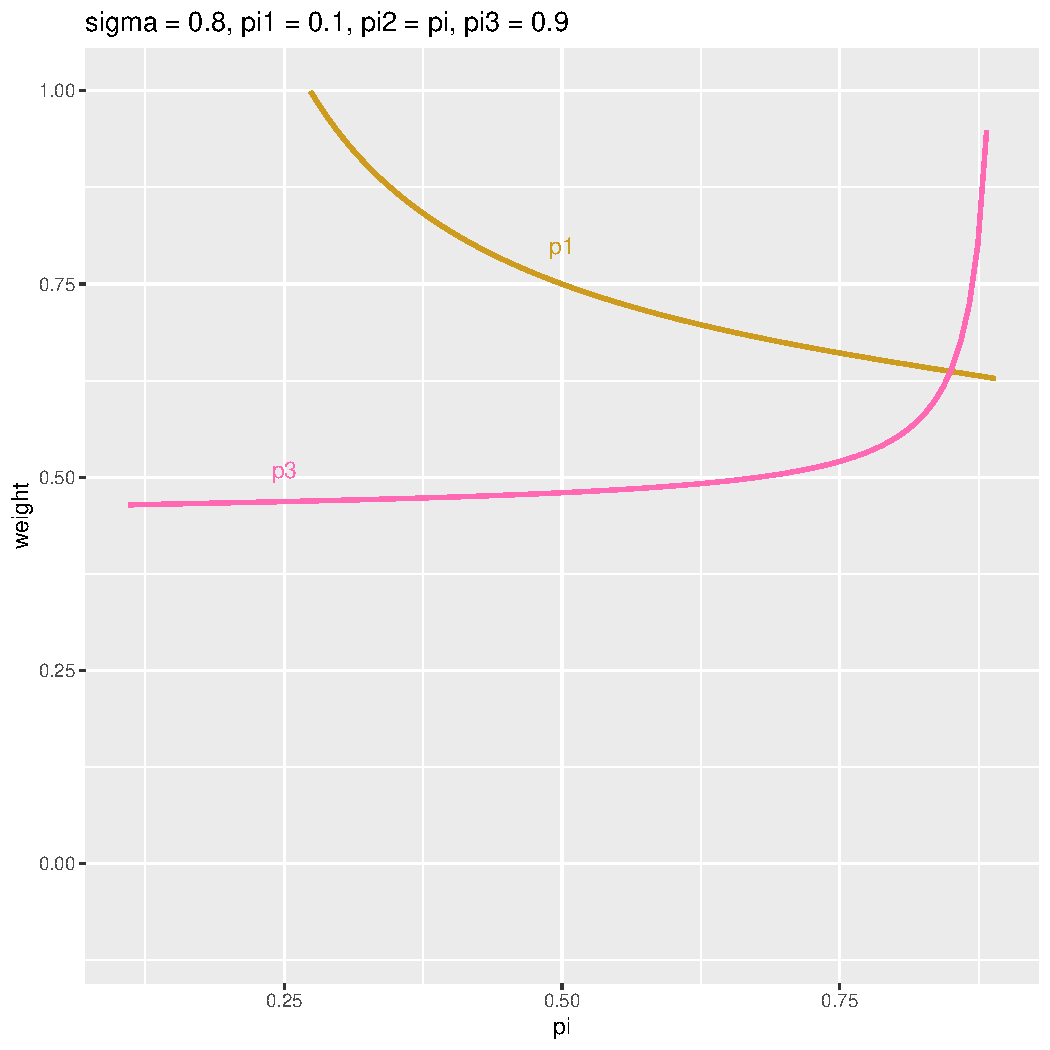
\includegraphics[width=1\linewidth]{img/p123_2.pdf}
			\caption{Веса $p_{1}$, $p_{2}$, $p_{3}$ в зависимости от $\pi$. } %% подпись к рисунку
			\label{ris11} %% метка рисунка для ссылки на него
		\end{minipage}
	\end{center}
\end{figure}

Теперь пусть $\pi_{1} = \pi$, $\pi_{2} = 0.5$, $\pi_{3} = 0.9$. Видим, что веса являются вероятностями при  $0 \leq \pi \leq 0.02$.

\begin{figure}[!hhh]
	\begin{center}
		\begin{minipage}[h]{0.95\linewidth}
			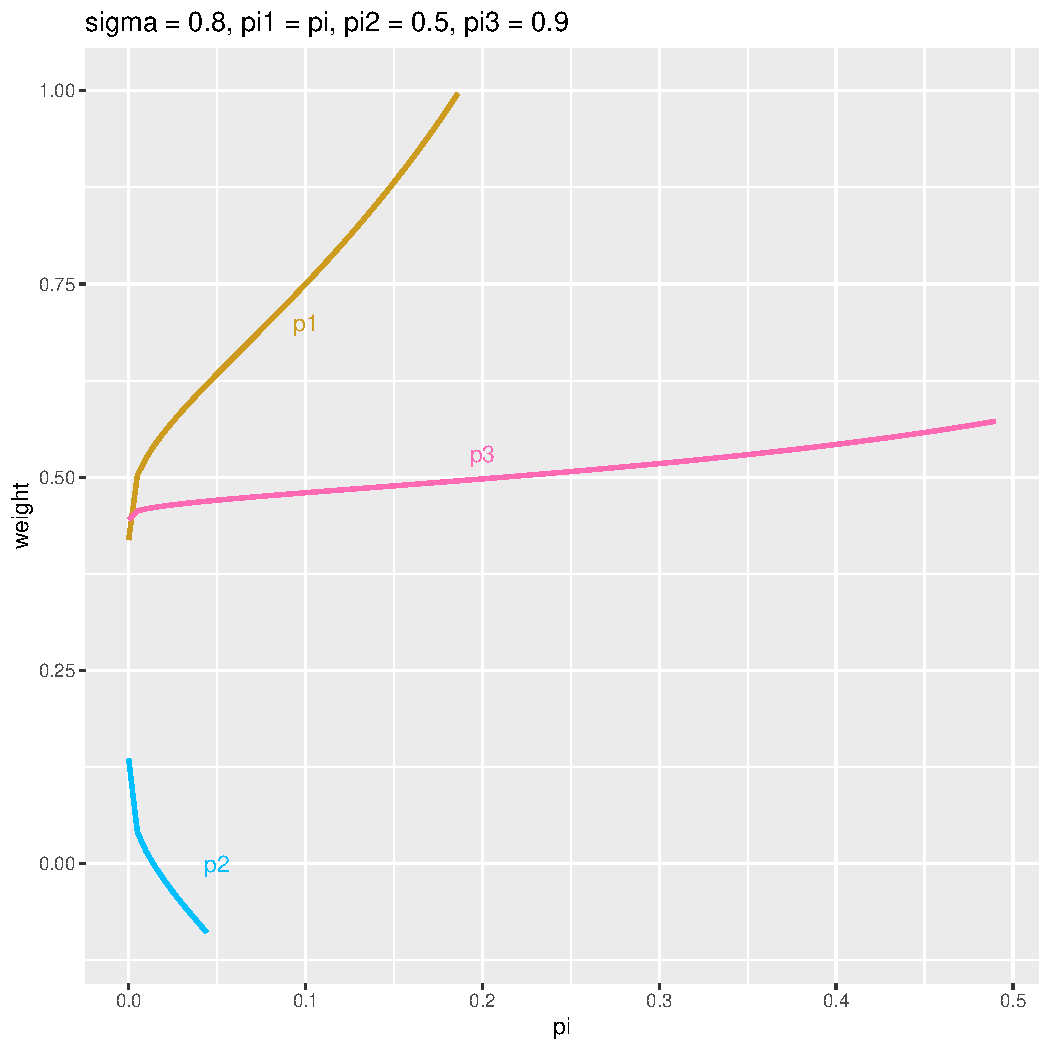
\includegraphics[width=1\linewidth]{img/p123_3.pdf}
			\caption{Веса $p_{1}$, $p_{2}$, $p_{3}$ в зависимости от $\pi$. } %% подпись к рисунку
			\label{ris11} %% метка рисунка для ссылки на него
		\end{minipage}
	\end{center}
\end{figure}

Теперь построим график зависимости верхней границы для $\sigma$ от $\pi$ для $\pi_{1} = 1-\pi$, $\pi_{2} = 0.5$, $\pi_{3} = \pi$ и для $\pi_{1} = 0.1$, $\pi_{2} = 0.5$, $\pi_{3} = \pi$. Он представлен на рисунке 10, видим, что $0 \leq \sigma \leq 1.5$ при $\pi = 0.98$. До значения $\sigma = 1.5$ быстрее доходит зеленая линия, то есть в случае $\pi_{1} = 0.1$, $\pi_{2} = 0.5$, $\pi_{3} = \pi$.

\begin{figure}[!hhh]
	\begin{center}
		\begin{minipage}[h]{0.95\linewidth}
			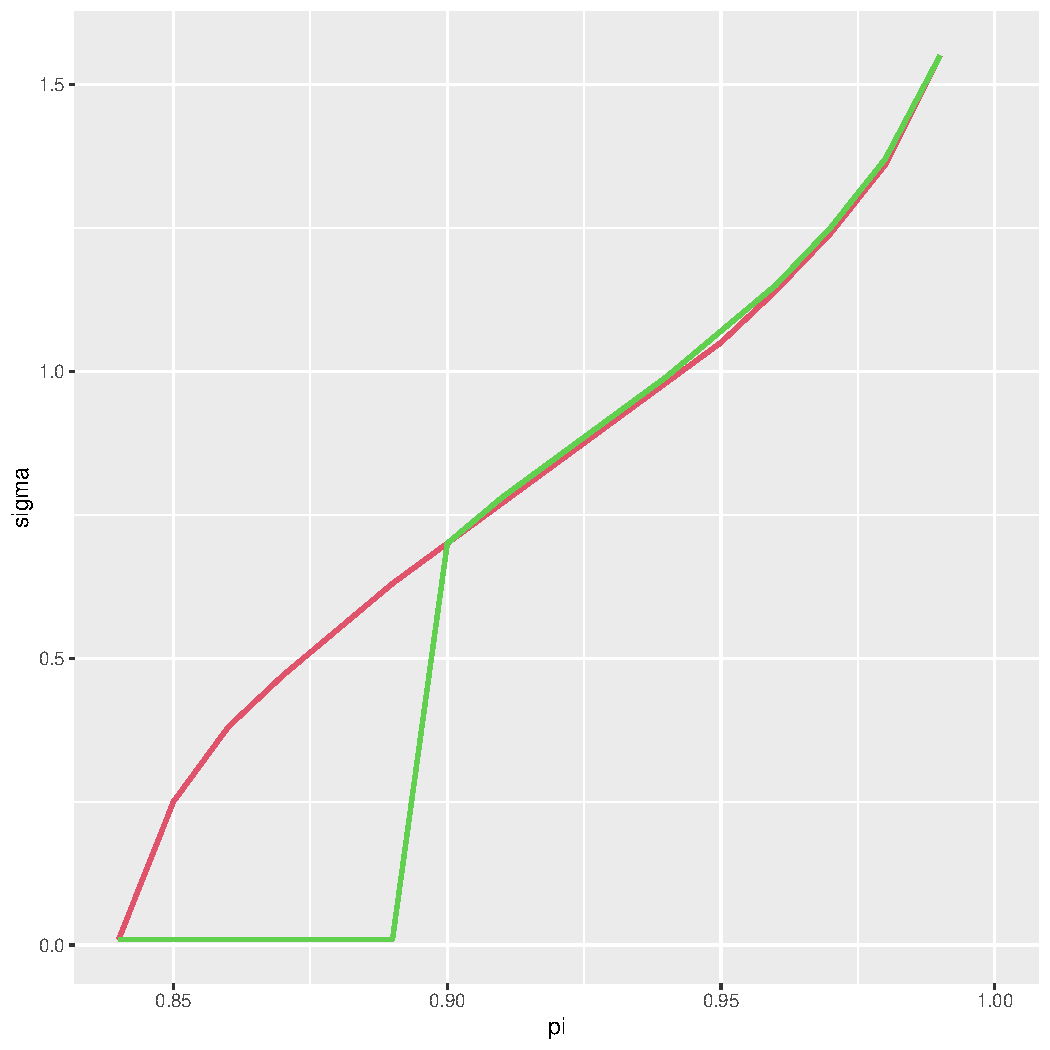
\includegraphics[width=1\linewidth]{img/sigma_12.pdf}
			\caption{Граница для $\sigma$ при $\pi_{1} = 1-\pi$, $\pi_{2} = 0.5$, $\pi_{3} = \pi$ (красный), при $\pi_{1} = 0.1$, $\pi_{2} = 0.5$, $\pi_{3} = \pi$ (зелёный). } %% подпись к рисунку
			\label{ris12} %% метка рисунка для ссылки на него
		\end{minipage}
	\end{center}
\end{figure}


	\clearpage
	\section{Заключение}
	
	Таким образом, мною были получены следующие результаты. 
	
	Получено условие на $\sigma$ для существования трехточечной симметричной аппроксимации логнормального распределения.
	Численно оценена точность аппроксимации мат. ожидания и дисперсии логнормального распределения с помощью метода Свонсона, применяемого к нормальному распределению.
	Построен алгоритм для нахождения трехточечной симметричной аппроксимации суммы логнормальных распределений.
	Численно оценена точность трехточечной аппроксимации суммы логнормальных распределений.
	
	\addcontentsline{toc}{section}{8\quad Список литературы}
	\begin{thebibliography}{1}
		\bibitem{Swansong} Keith G. Swanson's Swansong."--- Текст: электронный // stochastic: [сайт]."--- URL: https://www.stochastic.dk/post/swanson-s-swansong (дата обращения: 23.12.2021).
		
		\bibitem{Uncertainties} Uncertainties impacting reserves, revenue, and costs"--- Текст: электронный // AAPG Wiki: [сайт]."--- URL: https://wiki.aapg.org/Uncertainties impacting reserves, revenue, and costs (дата обращения: 27.05.2022).
		
		\bibitem{Discretization} Bickel, J. Eric, Lake, Larry W., and John Lehman. "Discretization, Simulation, and Swanson's (Inaccurate) Mean." SPE Econ Mgmt 3 (2011): 128–140. doi: https://doi.org/10.2118/148542-PA.
		
		\bibitem{Simulation} Bickel, J. Eric. "Discretization, Simulation, and the Value of Information." Paper presented at the SPE Annual Technical Conference and Exhibition, Denver, Colorado, USA, October 2011. doi: https://doi.org/10.2118/145690-MS.
		
		\bibitem{Performance} Moghadasi, Maryam and Jerry L. Jensen. “Performance Evaluation of Swanson’s Rule for the Case of Log-Normal Populations.” (2014). DOI:10.1007/978-3-642-32408.
		
		
	\end{thebibliography}
	
	
	
	
	
\end{document}